\chapter{The System}
\section{System Description}
At the ATF2 IP, inside the vacuum chamber, the BPMs positioning system has been installed during the first two weeks of July 2013.
It will move two blocks:
\begin{itemize}
\item BLOCK BPMs AB
\item BLOCK BPM C
\end{itemize}
This movement has two degrees of freedom: vertical (y) and lateral (x), both transverse to the beam direction. Beam crosses BPMAB first, then and empty space where Shintake monitor laser will be aligned, then crosses BPMC and goes out of the vacuum chamber.

These two blocks of BPMs, moving in two directions each, are displaced by Piezo-Movers (or just movers) made by different companies. German «PI electronics« moves  BPMC and French «Cedrat Technologies« moves BPMAB.

Each block has 3 vertical and one lateral movers. Lateral is underneath. Four movers are used per block, eight in total.

\section{The Piezo Movers}
Piezo mover changes its position as a function of voltage. Each one of the eight movers has its own control electronics block composed of: 
\begin{itemize}
 \item the mover
\item the strain gauge
\item the control box (manufacturer module) to:
\begin{itemize}
 \item set piezo mover voltage (high voltage)
 \begin{itemize}
\item PI module E-621
\item CEDRAT module LA75
\end{itemize}
\item read strain gauge
\begin{itemize}
\item PI module E-621 (same as control)
\item CEDRAT module SG75
\end{itemize}
\item set feedback operation (ON/OFF)
\item set control mode (external control from PLC is used)
\end{itemize}
\item PLC channel to
\begin{itemize}
\item set control voltage values equivalent to piezo mover displacement
\item read voltage values equivalent to strain gauge deformation
\end{itemize}
\end{itemize}

\subsection{Mover range}
PI and Cedrat have different ranges: PI (300um), Cedrat (250um)\par

Control voltage and its relation with displacement (min-max) varies between both companies:\par
\begin{itemize}
\item PI: 		(min)   0V   	to 	(max) 10V
\item CEDRAT: 	(max) -1V 	to	(min)    7V
\end{itemize}
It is important to note that:
\begin{itemize}
\item The voltage-displacement relation is inverse for CEDRAT movers.
\item When the system is OFF (0V), PI mover are at its minimum, however CEDRAT are not.
\end{itemize}

\subsection{Mover Control}
Control per mover\par
\begin{center}
\begin{tikzpicture}
 \node (img1) {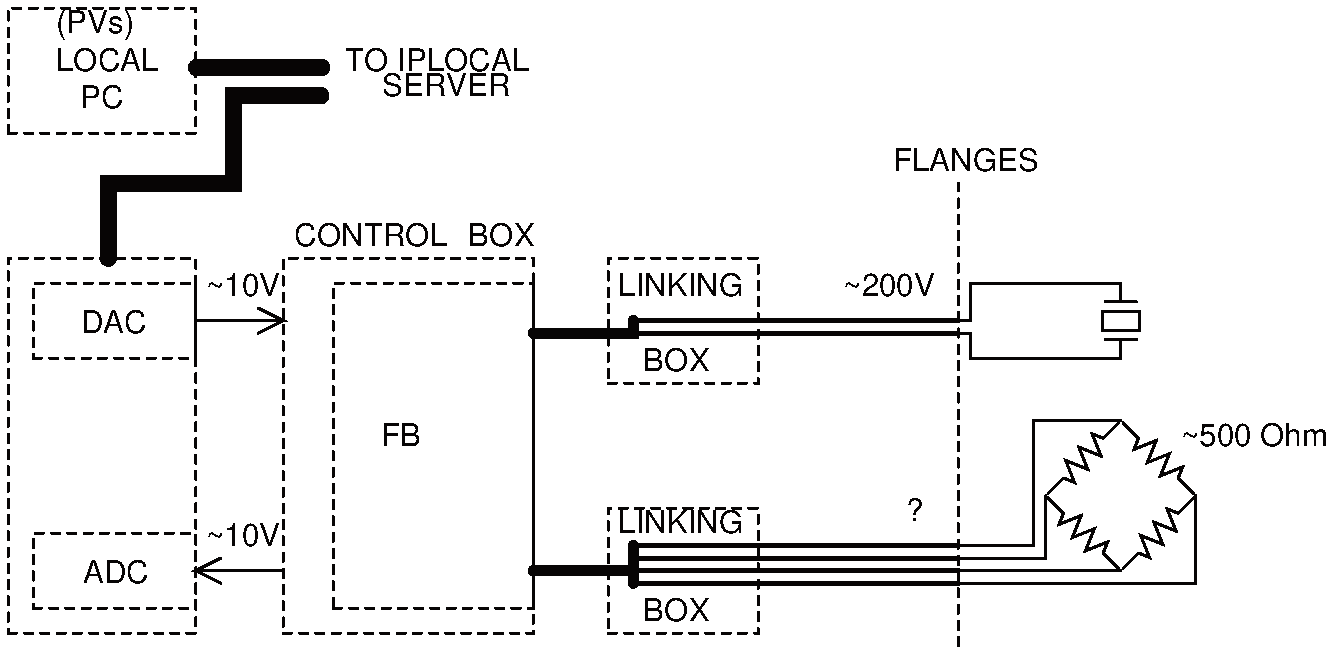
\includegraphics[scale=0.5]{Page1.pdf}};
 %\node (img2) at (4.4,1.5) {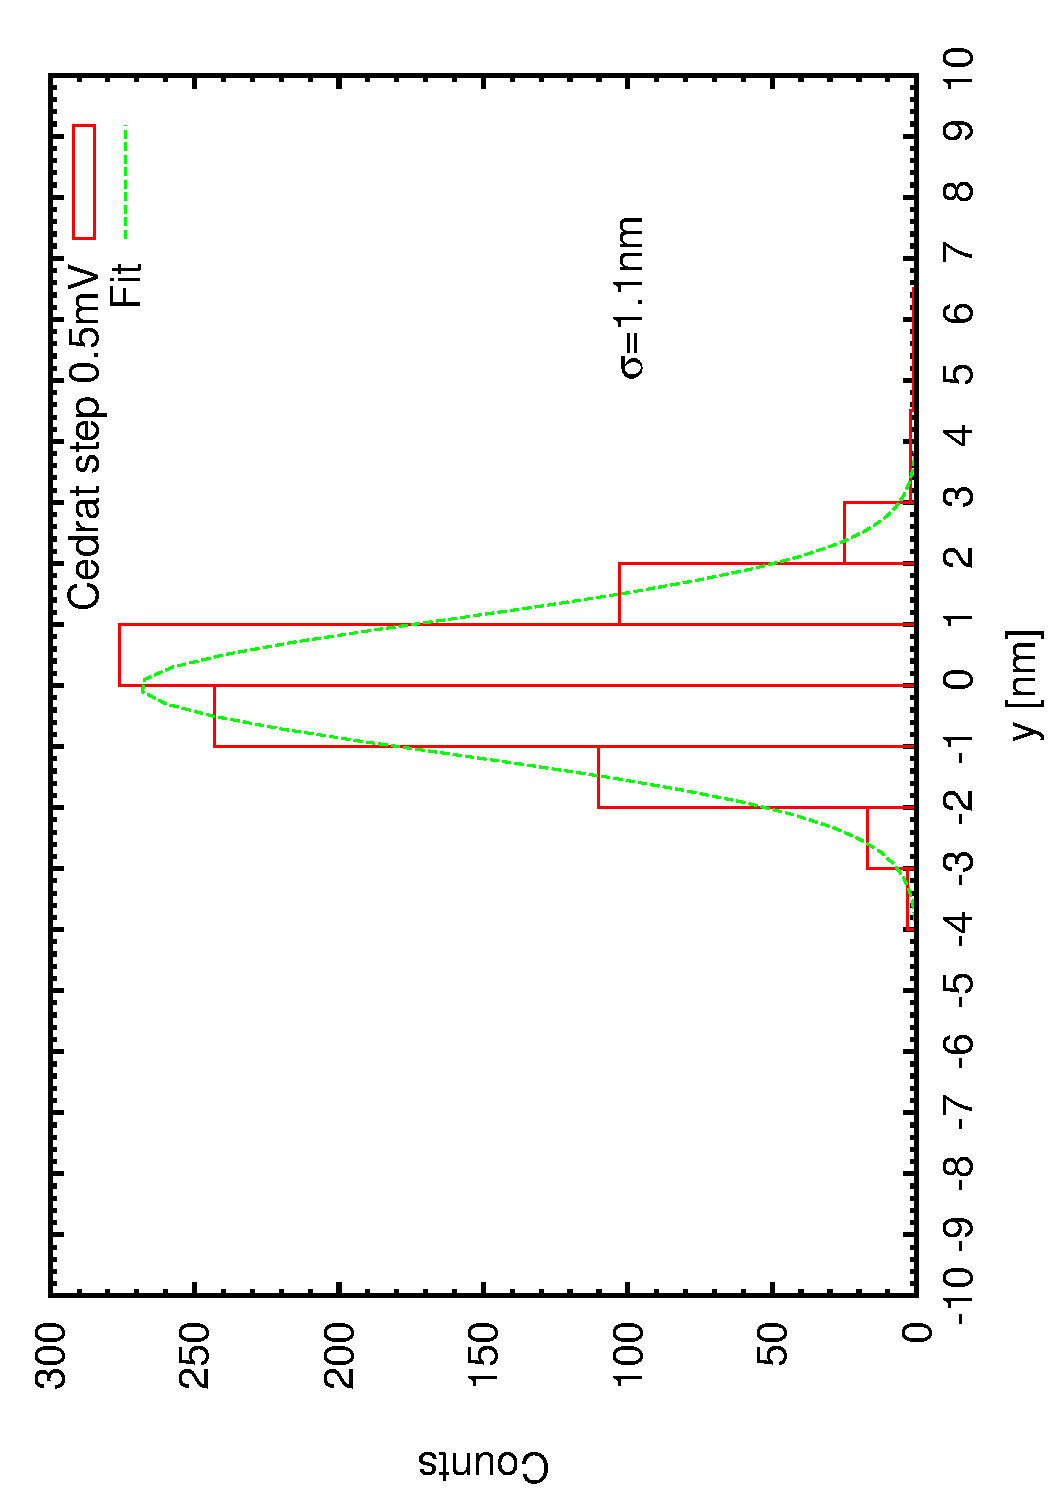
\includegraphics[scale=0.1,angle=-90]{imagestep12.pdf}};
%  \node (img3) at (4.4,2.6) {$\sigma_y=$?};
 %\node (img3) at (4.4,1.5) {{\LARGE\color{red} ?}};
\end{tikzpicture}
\end{center}
{\tiny BLOCK AB 1mV=31.25nm, BLOCK C 1mV=30nm}\par

\subsection{Feedback and NO Feedback}
There are two operation possibilities per mover: Feedback (fb) and No Feedback (no fb). It means 8 feedback loops. On each case the control module sets a voltage value on the mover and read the strain gauge to create a closed loop. However, their implementations are different on each company.

\section{The PLC}
Two NI9263 are used to set analogue voltage into the mover control electronics. Two NI9239 are used to read analogue voltage from the strain gauge readback. One NI9219 is used to read temperature. These modules are connected to the chassis NI9188 which is connected by network to a working station with Labview installed.
The block chassis+NI modules is called \textbf{PLC}.\par
\textbf{National instruments Chassis: NI9188}
\begin{itemize}
\item Mac Address: 0080.2f14.b777
\item DHCP
\item IP address (ATF) 31.1.1.39
\item IP address (KEK): None
\item Host name: ipmv-plc.ip-local
\item Net Mask: 255.255.255.0
\item connected to ip-local during installation
\end{itemize}
Chassis NI9188 can connect up to 8 modules, not all are used:
\begin{itemize}
\item PI
\begin{itemize}
\item Module 5: NI9263 Digital to analogue converter
\item Module 6: NI9239 Analogue to digital converter
\end{itemize}
\item Cedrat
\begin{itemize}
\item Module 2: NI9263 Digital to analogue converter
\item Module 3: NI9239 Analogue to digital converter
\end{itemize}
\item Temperature
\begin{itemize}
\item Module 8: NI9219 Temperature probes
\begin{itemize}
\item Cedrat: 	Channel 0
\item PI: Channel 2
\end{itemize}
\end{itemize}
\item The other slots are not used
\end{itemize}

\section{The PC}
It is used to control from close locations the BPM positioning system. It sets the digital values to put in the PLC and reads the digital values from the PLC channels corresponding to strain gauges.\par
\subsection{Characteristics}
LAL Computer (Laptop)\par
Processor Inter Core i7 vPro\par
Mac Address: d067.e550.620e\par
DHCP\par
IP address(ATF): 31.1.1.38\par
IP address (KEK): Wifi connection (MAC registered at KEK)\par
Net Mask: 255.255.255.0\par
connected to ip-local during installation\par

\subsection{Used Software}
Windows 7 Français\par
National Instrument - Labview 2011\par
National Instruments - Measurement $\&$s Automation Explorer (NI MAX)\par
Gimp 2.8\par
Microsoft office – Excel 2013\par
cmd\par
Highly Dynamic and Precise motion 45 V 1.6 (HDPM45V16)– Cedrat Technologies\par
\subsection{Folder Content Description}\par
Path to applications and info\par
\verb?Bureau/Actionneurs Piezo/Applis?\par
All applications were done in Labview. Filenames gives a hint of its content (keywords used in filenames):\par
\begin{itemize}
\item \verb?oscilloscope?: uses de ADC to read signals
\item \verb?generateur?: function generator, uses de DACs to produce signals
\item \verb?Actionneurs positionnement BPMs?: activate the system displacement
\item \verb?Ethernet?: connected by wired network,
\item \verb?USB?: corresponds to previous version connected by USB.
\item \verb?Verticaux groupe?: all 3 vertical mover movers are activated by one voltage control
\item \verb?mouvements identiques?: first version of BPM displacement system (PI and CEDRAT) integrated.
\item \verb?Jauges?: stores the strain gauges info in excel format.
\item \verb?temp?: stores temperature info in excel format.
\item \verb?epics?: control from epics system, Labview works as interface.
\item \verb?Actionneurs multicycles?: several cycles over the defined voltage range are performed
\item \verb?Cedrat, PI?: identifies the group of movers to use.
\item \verb?Vertical, lateral fixe?: it means that one direction of movement is set (fixed) to a voltage value while the other direction varies in cycles.
\end{itemize}

\subsection{Access}
Account: **********(not in this document)\par
Password: *********(not in this document)\par

\subsection{PVs}
Epics PVs (Process Variables). Write: sets a value on the DAC. Read: reads from ADC.\par
Channels IP:BPM-AB:Mover0 and IP:BPM-C:MoverB are for lateral movement.\par
IP:BPM-AB:Mover0:Read\par
IP:BPM-AB:Mover0:Write\par
IP:BPM-AB:Mover1:Read\par
IP:BPM-AB:Mover1:Write\par
IP:BPM-AB:Mover2:Read\par
IP:BPM-AB:Mover2:Write\par
IP:BPM-AB:Mover3:Read\par
IP:BPM-AB:Mover3:Write\par 
IP:BPM-C:MoverB:Read\par 
IP:BPM-C:MoverB:Write\par 
IP:BPM-C:MoverC:Read\par 
IP:BPM-C:MoverC:Write\par 
IP:BPM-C:MoverD:Read\par 
IP:BPM-C:MoverD:Write\par 
IP:BPM-C:MoverE:Read\par 
IP:BPM-C:MoverE:Write\par 
IP:BPM-AB:Temp\par 
IP:BPM-C:Temp\par 
\vspace*{0.5cm}
Older Epics PVs, DO NOT USE (Process Variables)\par 
These PVs are here for documentation purposes. They are still functional but any new work should be done with previously defined PV in this document.\par 
Write: sets a value on the DAC.\par 
Read: reads from ADC.\par 
Channels Cedrat0 and PIB are for lateral movement.\par 
IPBSM:BPMs:PIB:Write\par 
IPBSM:BPMs:PIB:Read\par 
IPBSM:BPMs:PIC:Write\par 
IPBSM:BPMs:PIC:Read\par 
IPBSM:BPMs:PID:Write\par 
IPBSM:BPMs:PID:Read\par 
IPBSM:BPMs:PIE:Write\par 
IPBSM:BPMs:PIE:Read\par 
IPBSM:BPMs:Cedrat0:Write\par 
IPBSM:BPMs:Cedrat0:Read\par 
IPBSM:BPMs:Cedrat1:Write\par 
IPBSM:BPMs:Cedrat1:Read\par 
IPBSM:BPMs:Cedrat2:Write\par 
IPBSM:BPMs:Cedrat2:Read\par 
IPBSM:BPMs:Cedrat3:Write\par 
IPBSM:BPMs:Cedrat3:Read\par 
Read temperature:\par 
IPBSM:BPMs:Temp1\par 
IPBSM:BPMs:Temp2\par

\section{The BPMs}
\subsection{Coordinate system}\par
Each BPM has its own coordinates with respect to a reference system centered \textbf{electrically} and aligned with the beam\par
\vspace*{0.5cm}
% \centering
\begin{minipage}{7cm}
  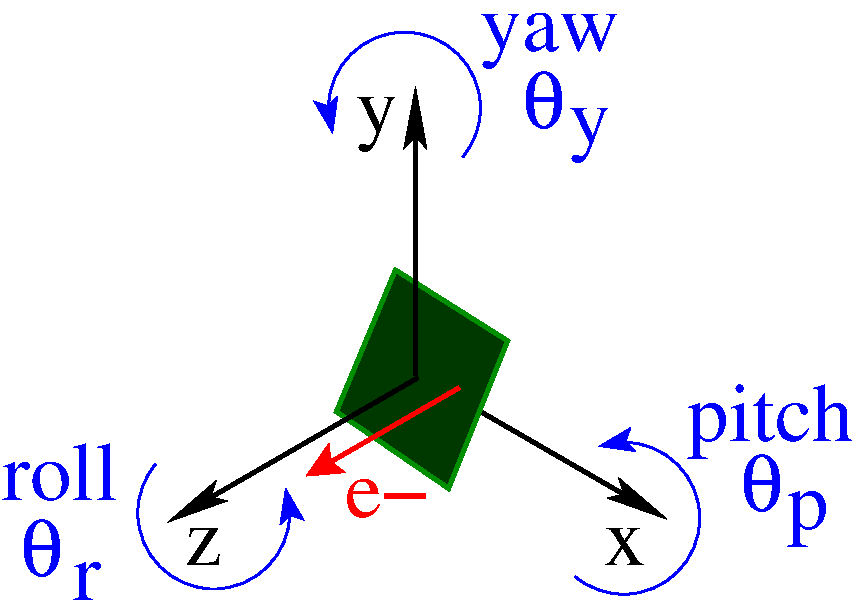
\includegraphics[scale=0.3,angle=0]{fig23.pdf}\\
  {\color{red}Beam}, {\color{forestgreen} BPMs}\\
\end{minipage}
\begin{minipage}{7cm}
\begin{itemize}
 \item Beam Position
 \\$x_A,y_A,z_A$\\$x_B,y_B,z_B$\\$x_C,y_C,z_C$
 \item BPM Angles respect to ref. system\\
 $\theta_{Ap},\theta_{Ar},\theta_{Ay}$\\
 $\theta_{Bp},\theta_{Br},\theta_{By}$\\
 $\theta_{Cp},\theta_{Cr},\theta_{Cy}$
\end{itemize}
\end{minipage}\par
All systems relate to a common \textbf{mechanical} reference system, no rotations, just translations\par
\centering
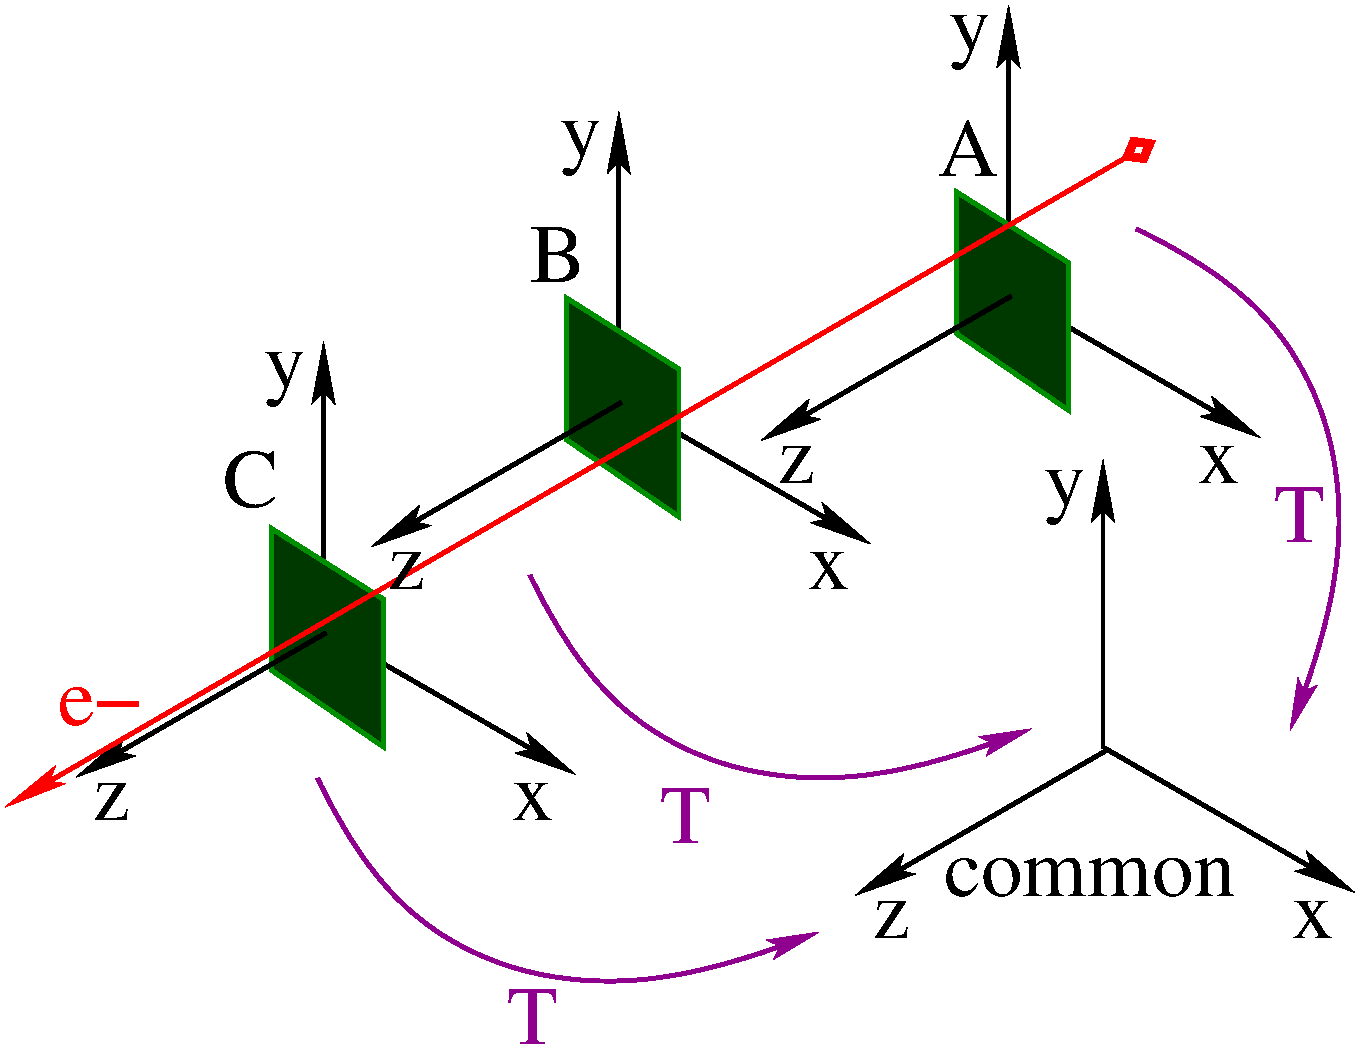
\includegraphics[scale=0.2,angle=0]{fig17.pdf}\\
\textbf{One of the BPMs reference system could be chosen to coincide with the common}\\
There is a set of movers to control BPM position\vspace{-0.5cm}
\centering
%\begin{columns}
%\begin{column}{3.5cm}
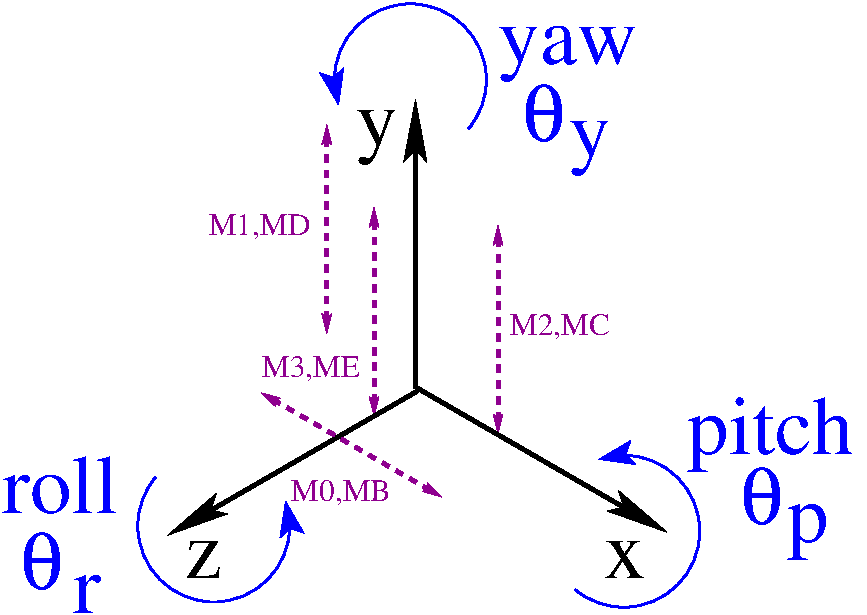
\includegraphics[scale=0.30,angle=0]{fig25.pdf} 
%\end{column}
%\begin{column}{5.5cm}
\begin{align*}
 x &= x_0+f_x(M_{0,B})\\
 y &= y_0+f_y(M_{123,CDE})\\
 z &= z_0\\
 \theta_p &= \theta_{p0}+f_p(M_{123,CDE})\\
 \theta_r &= \theta_{r0}\\
 \theta_y &= \theta_{y0}
\end{align*}\par
\vspace*{-0.4cm}All initial values are set during the IP BPMs installation\par
%\end{column}
%\end{columns}\vspace*{0.5cm}
%\begin{columns}
% \begin{column}{5cm}
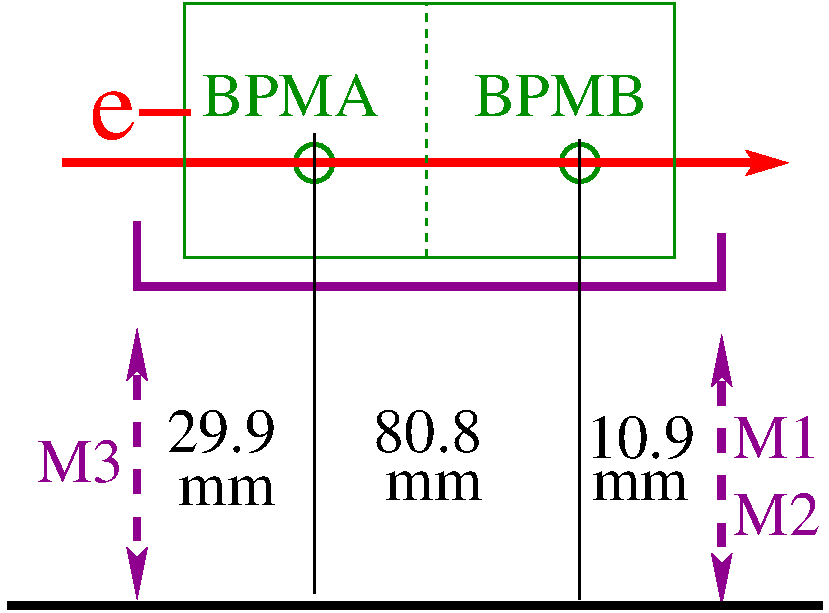
\includegraphics[scale=0.25,angle=0]{fig27.pdf}
% \end{column}
%\begin{column}{5cm}
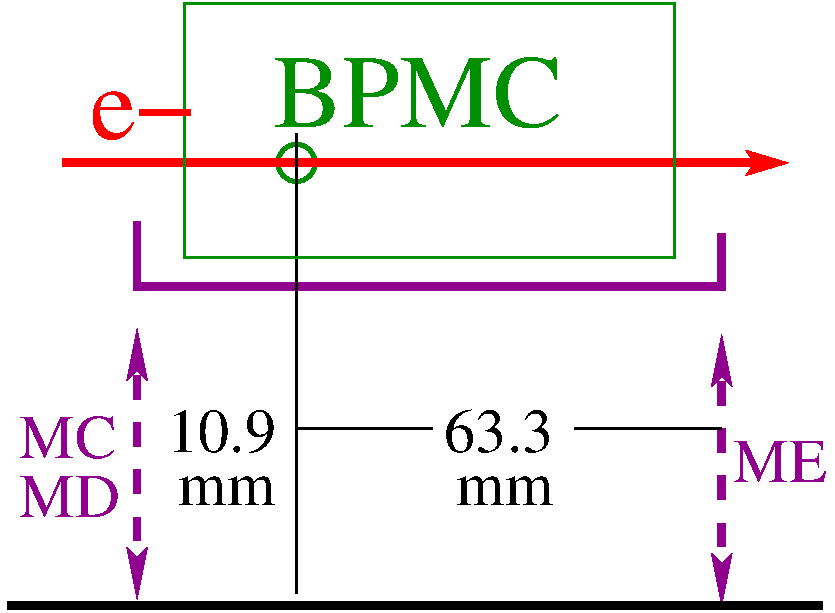
\includegraphics[scale=0.25,angle=0]{fig26.pdf}
% \end{column}
%\end{columns}
% \end{frame}
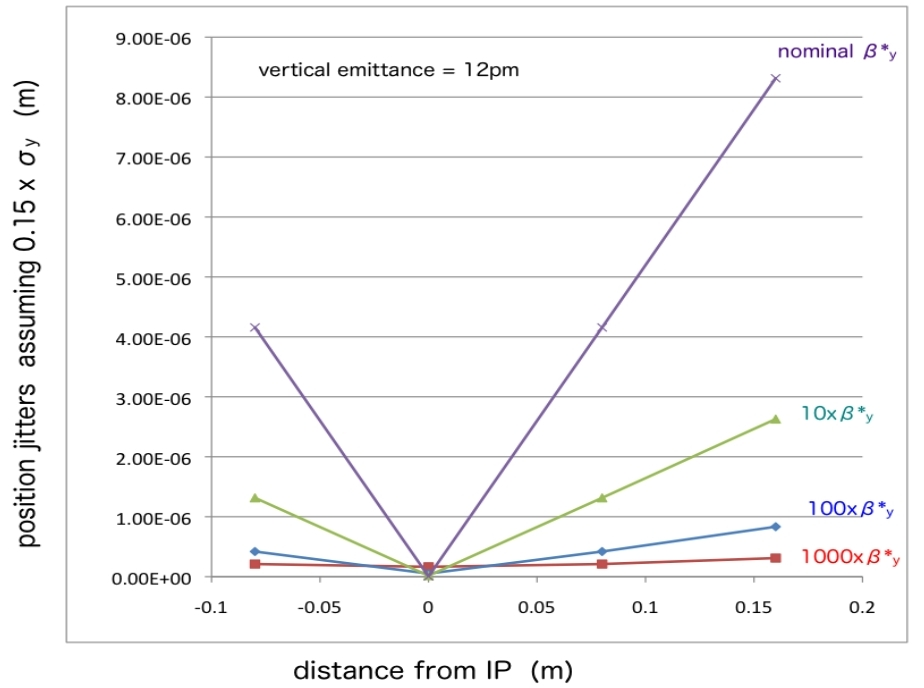
\includegraphics[scale=0.3,angle=0]{pos_beta2}
\raggedright

\subsection{Alignment adjustment}
\centering
\begin{equation}
 M_{0123}=\frac{3-V_{0123}[\text{V}]}{4} \qquad M_{BCDE}=\frac{V_{BCDE}[\text{V}]-5}{5}
\end{equation}
\begin{tabular}{|c||c|c|c|}\hline
 &\multicolumn{3}{|c|}{Adjustment}\\\cline{2-4}
 & B & A & C\\\hline\hline
$x$[$\mu$m] & $x_{0B}+{\color{magenta}125M_0}$ & $x_{0A}+{\color{magenta}125M_0}$&${x_{0C}+\color{magenta}150M_{B}}$\\
$y$[$\mu$m]& $y_{0B}+{\color{magenta}94.8M_{1,2}+30.2M_3}$&$y_{0A}+{\color{magenta}11.2M_{1,2}+113.8M_3}$&$y_{0C}+{\color{magenta}128.0M_{CD}+22.0M_E}$\\
$z$[mm]&$z_{0B}$&$z_{0B}-8.08$&$z_{0B}+$?\\
$\theta_{p}$[mrad]& $\theta_{p0B}+{\color{magenta}1.03(M_3-M_{1,2})}$ & $\theta_{p0A}+{\color{magenta}1.03(M_3-M_{1,2})}$ &$\theta_{p0C}+{\color{magenta} 2.02(M_{DC}-M_E)}$\\
$\theta_{r}$[mrad]&$\theta_{r0B}$&$\theta_{r0A}$&$\theta_{r0C}$\\
$\theta_{y}$[mrad]&$\theta_{y0B}$&$\theta_{y0A}$&$\theta_{y0C}$\\\hline
\end{tabular}\par
${\color{magenta} M_{0123,BCDE}}\in[-1,1],{\color{magenta}\Delta M_{0123,BCDE}}\geq1.25\times 10^{-2}$

\subsection{Sensitivity to angle (BPMA and BPMC)}
$1000\beta_y$ optics. 51 bunches recorded per each mover position. Maximum IQ value was picked each time.\\
\centering
 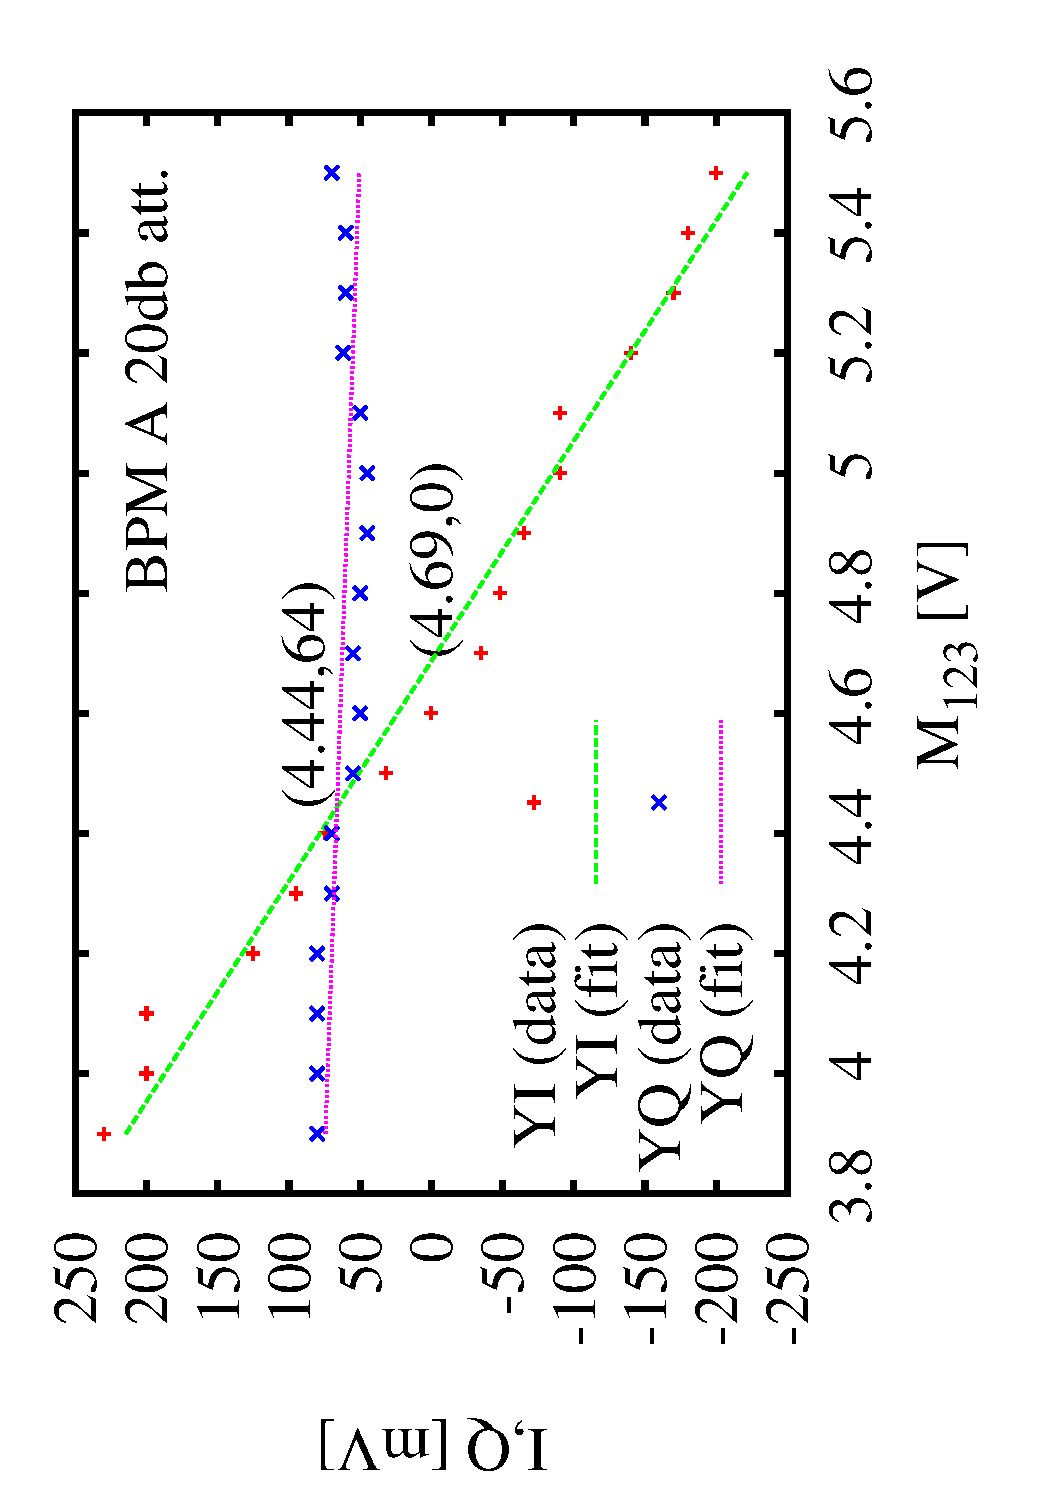
\includegraphics[scale=0.3,angle=-90]{image01_sense.pdf}\\
 \begin{equation}
  \text{Sensitivity to angle BPMA}<(4.69[\text{V}]-4.44[\text{V}])\left(\frac{250[\mu\text{m}]}{8[\text{V}]}\right)\left(\frac{1}{1.6[\text{mrad}]}\right)=4.9\left[\frac{\mu\textmd{m}}{\textmd{mrad}}\right]
 \end{equation}
 For BPMC, the result was 3.2 $\mu$m/mrad from FONT group. IP-BPM meeting 2014.03.26.
\raggedright

\section{Electrical connections}
\hspace*{1.4cm}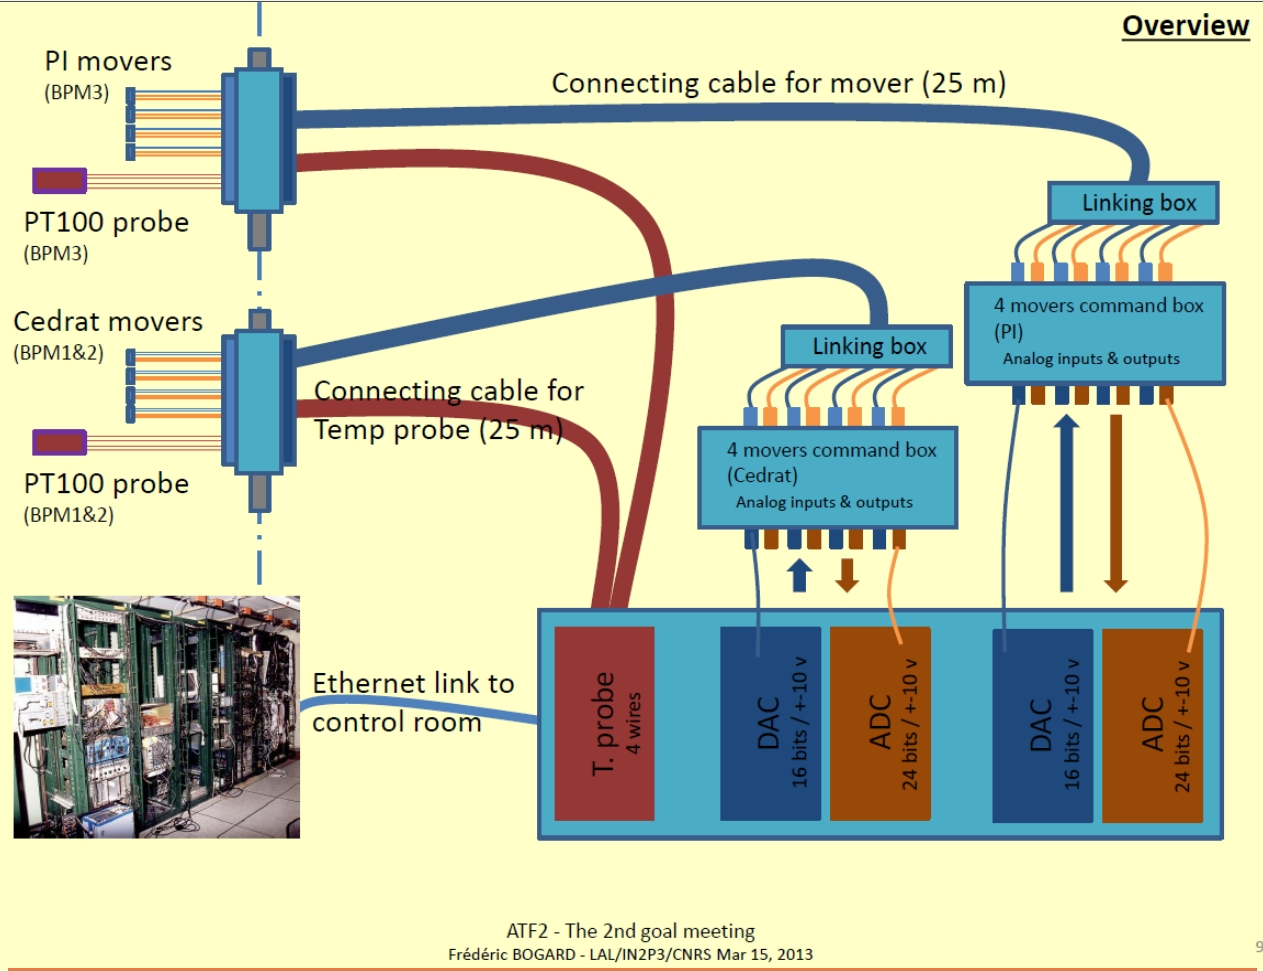
\includegraphics[angle=0,scale=0.2]{link.jpg}\par
%\hspace*{1.4cm}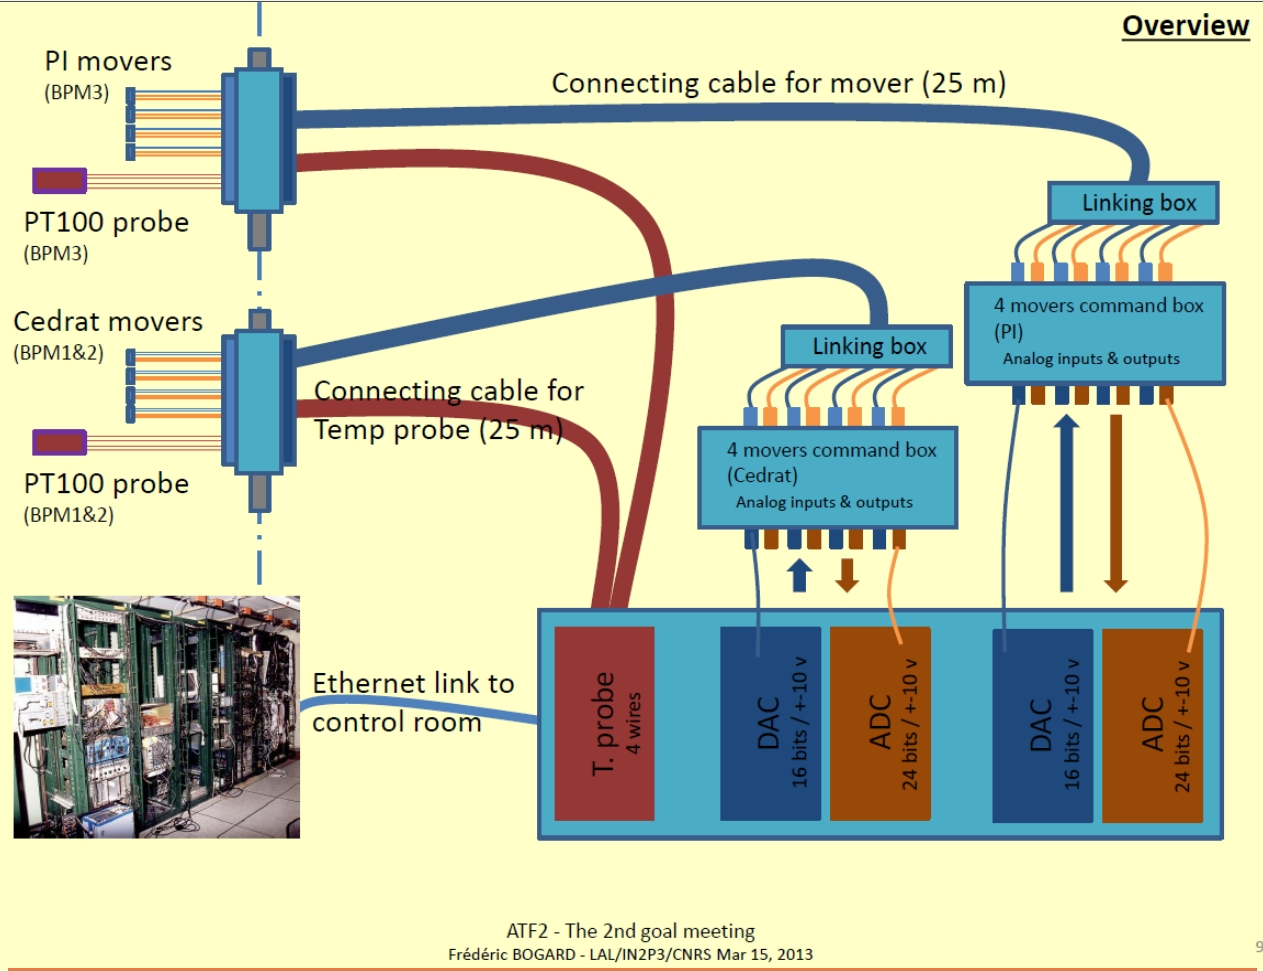
\includegraphics[angle=0,scale=0.2]{link.jpg}
\begin{tikzpicture}
  \node (img1) {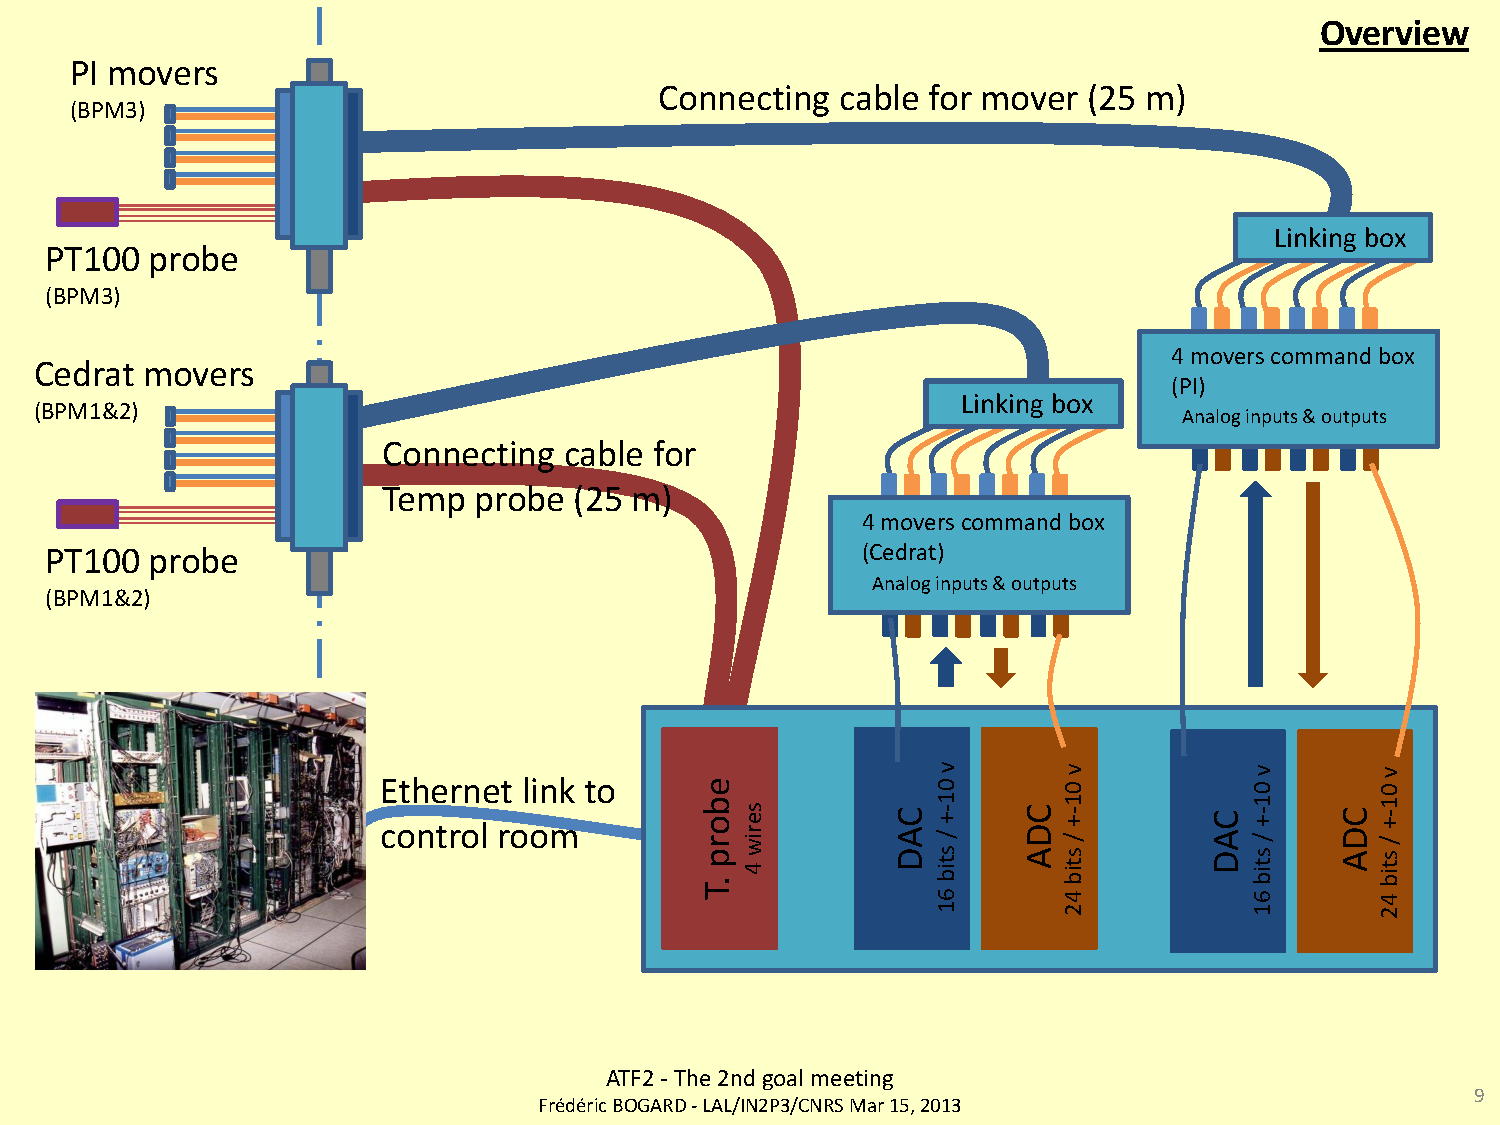
\includegraphics[scale=0.45,angle=0]{elect01.pdf}};
 %\pause
  \node (img2) at (-4.2,-3) {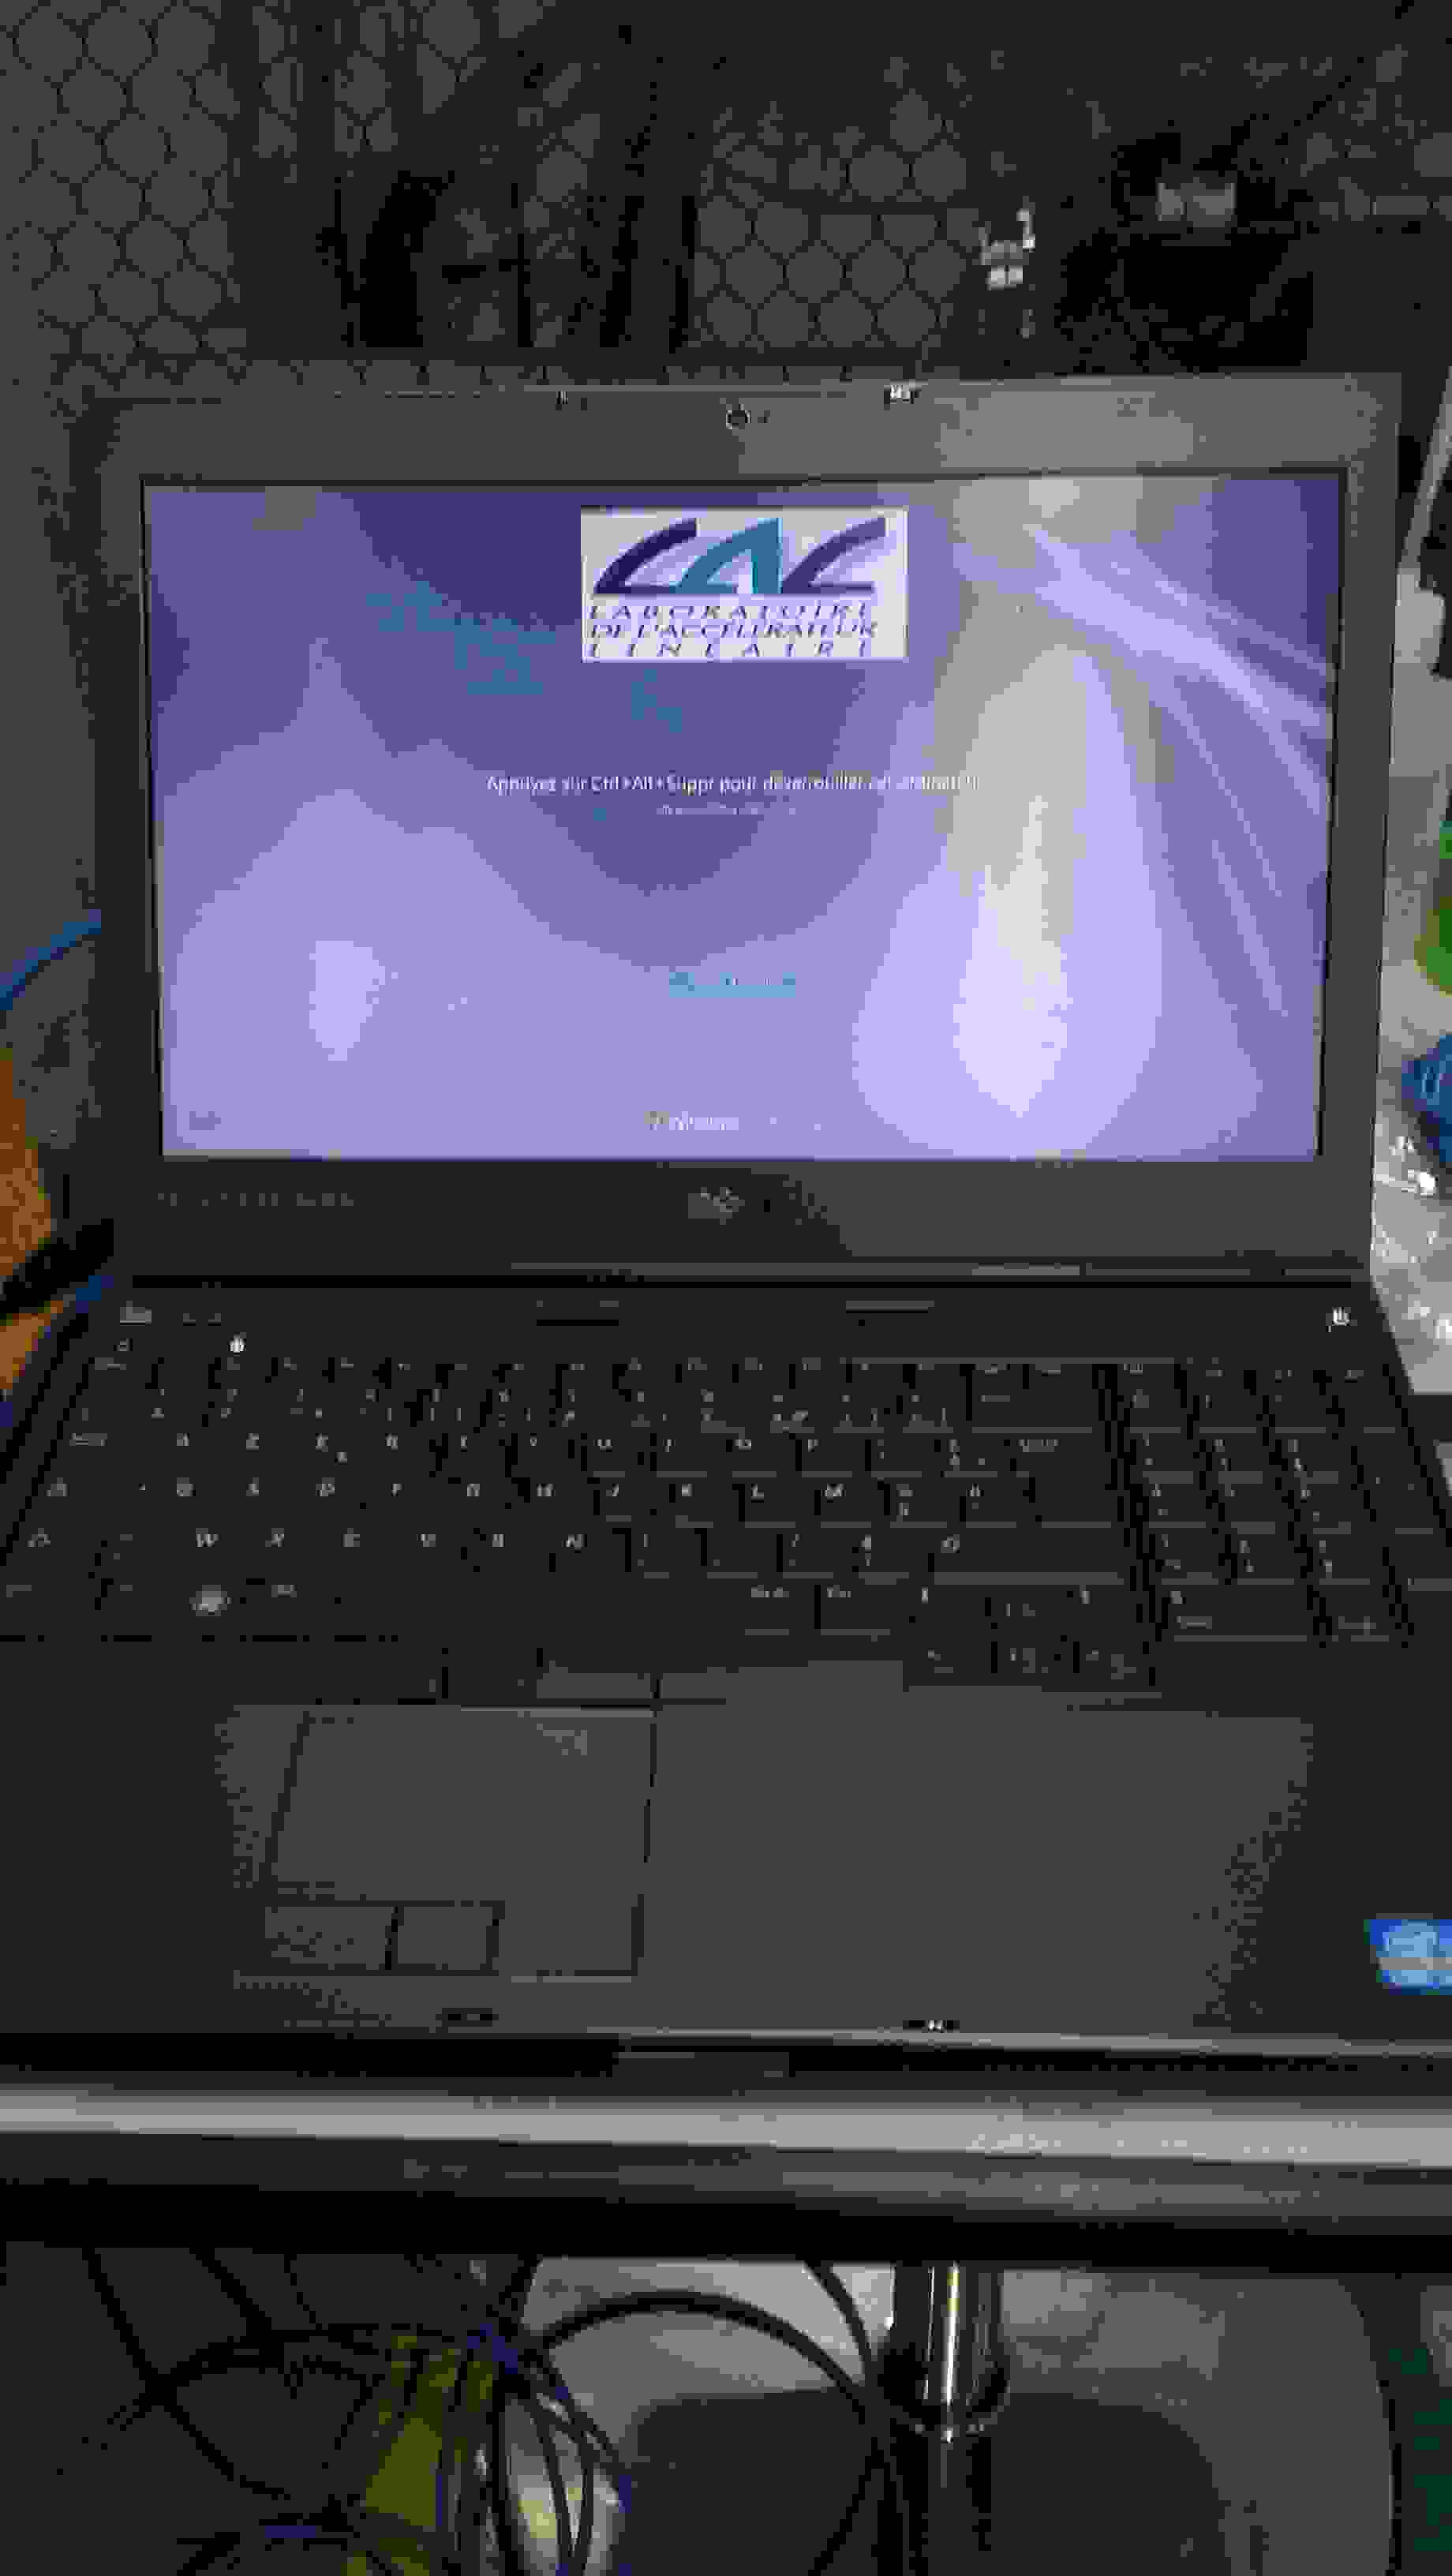
\includegraphics[scale=0.039,angle=0]{ima02a.jpg}};
%   \pause
  \node (img3) at (2.2,-2.1) {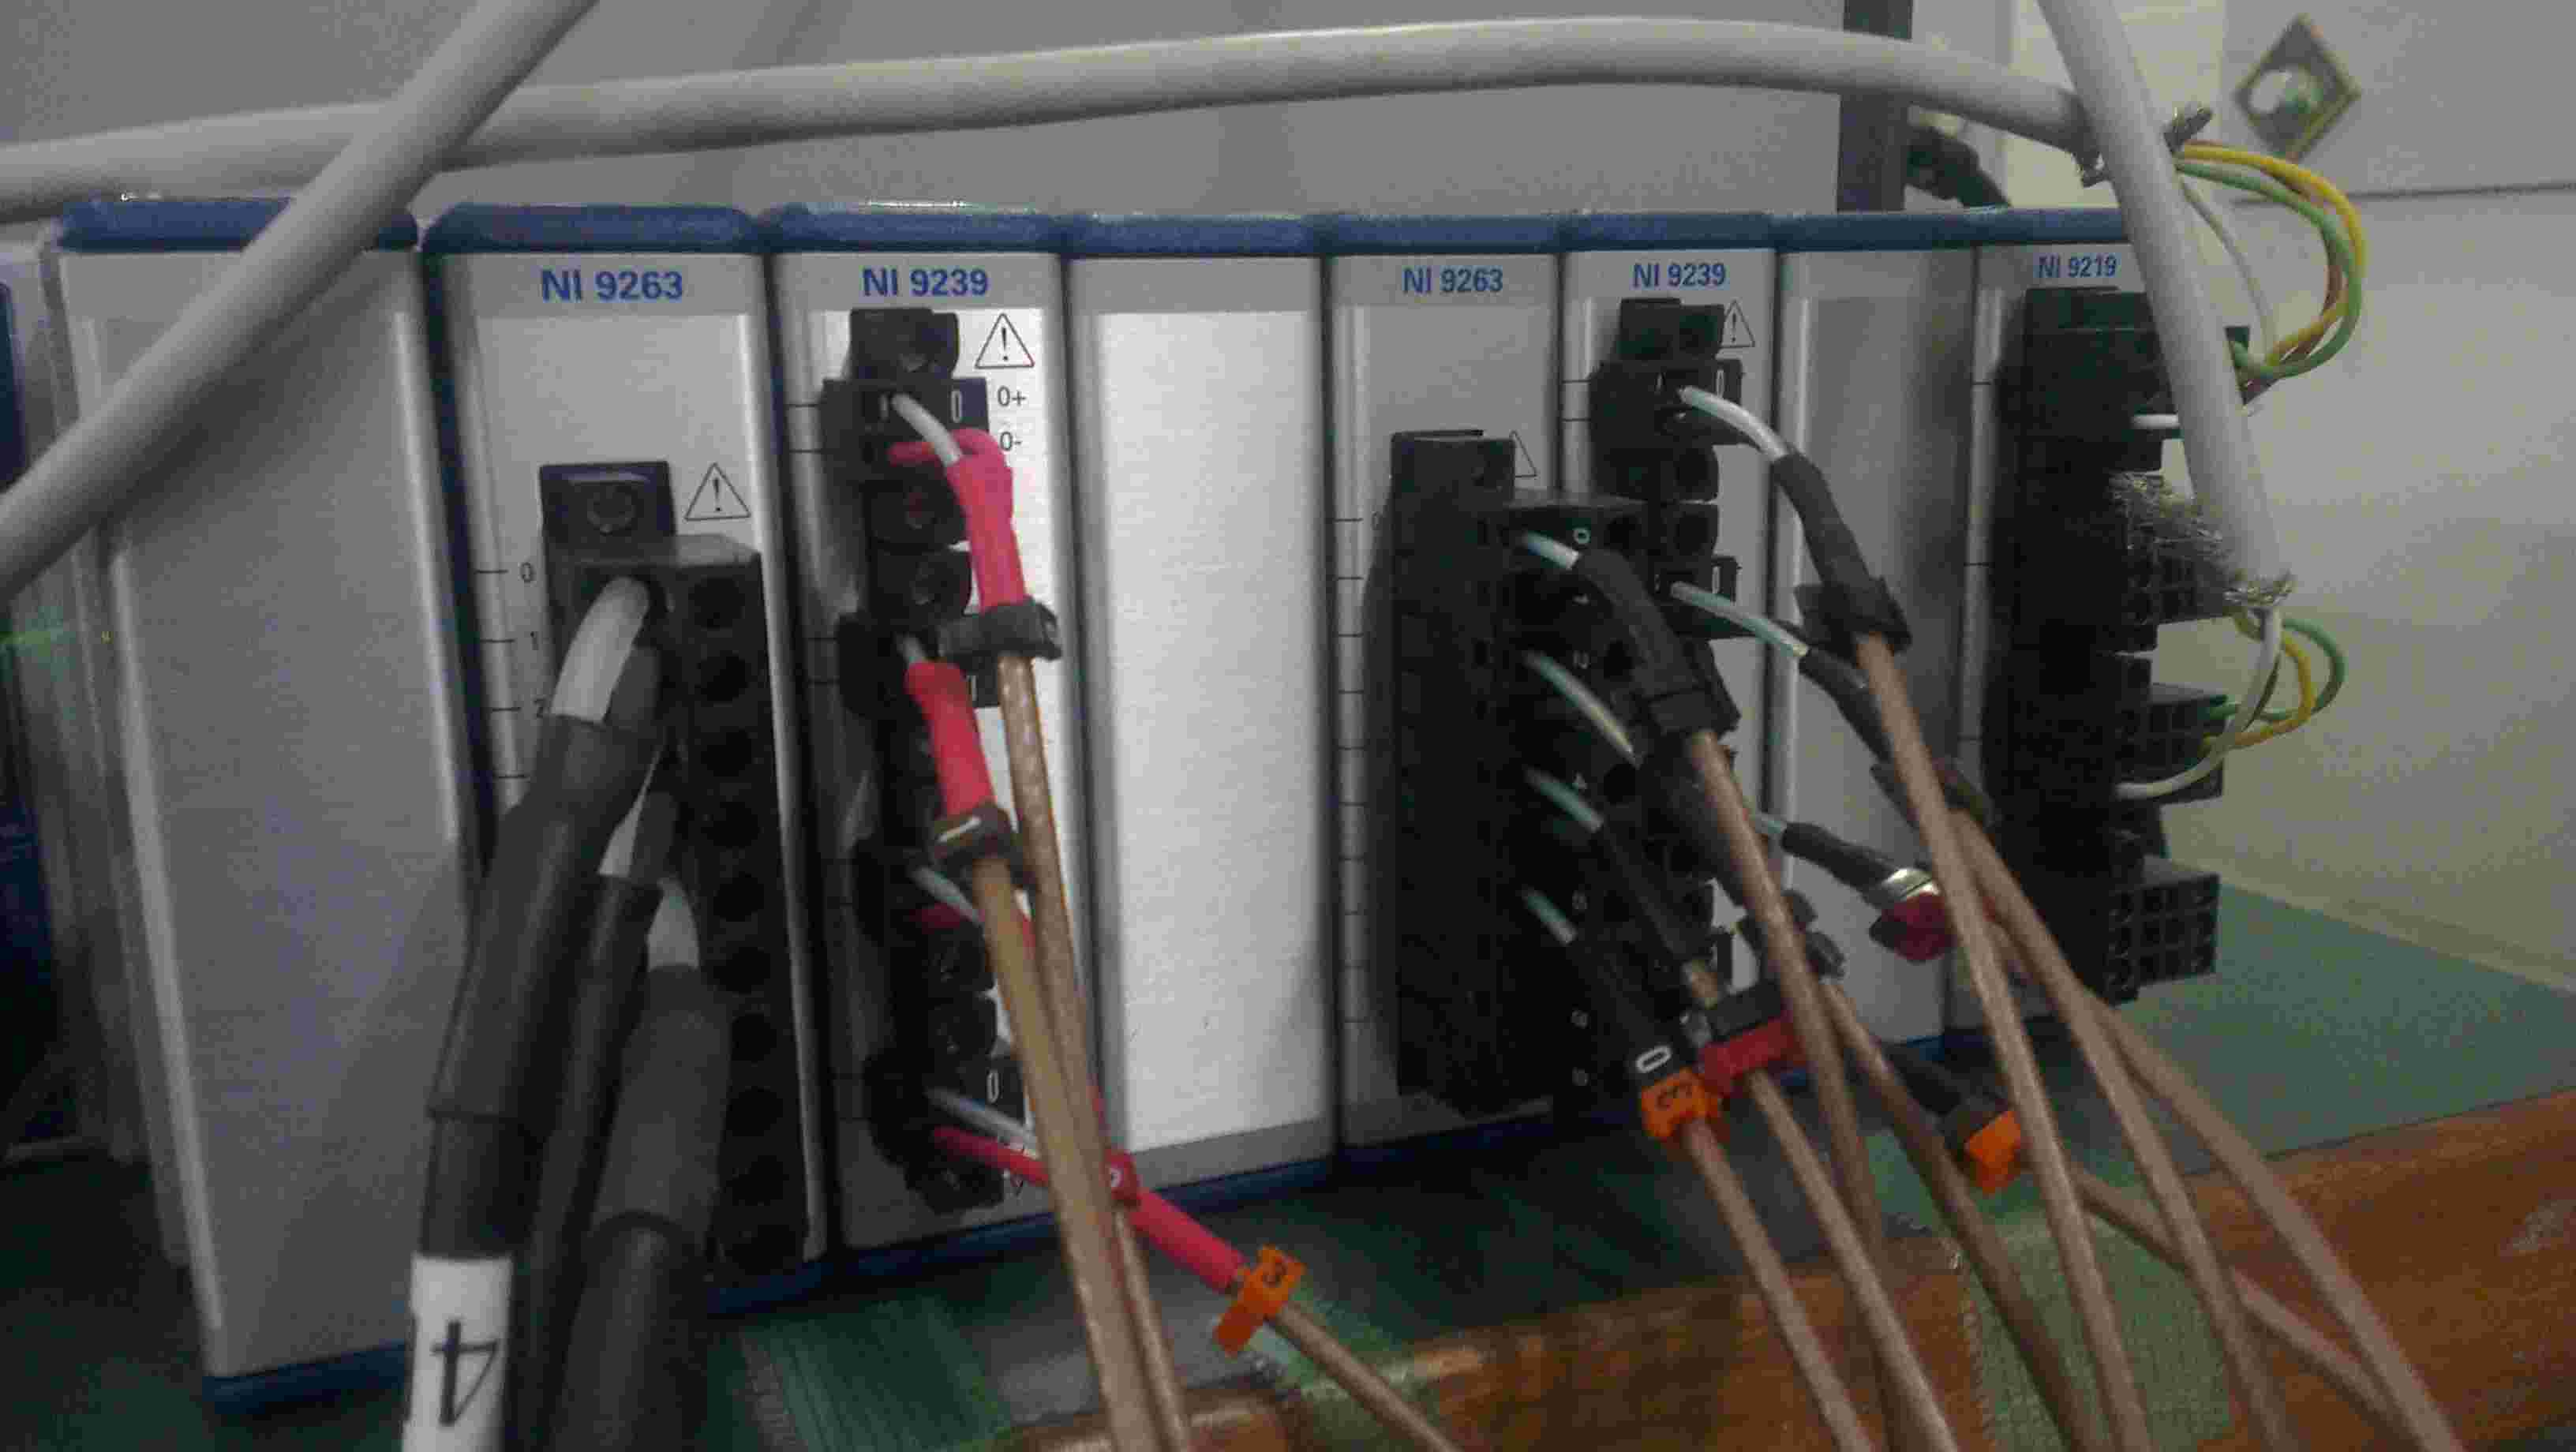
\includegraphics[height=2.5cm,width=6.2cm,angle=180]{ima06a.jpg}};
%   \pause
  \node (img4) at (4.4,1.0) {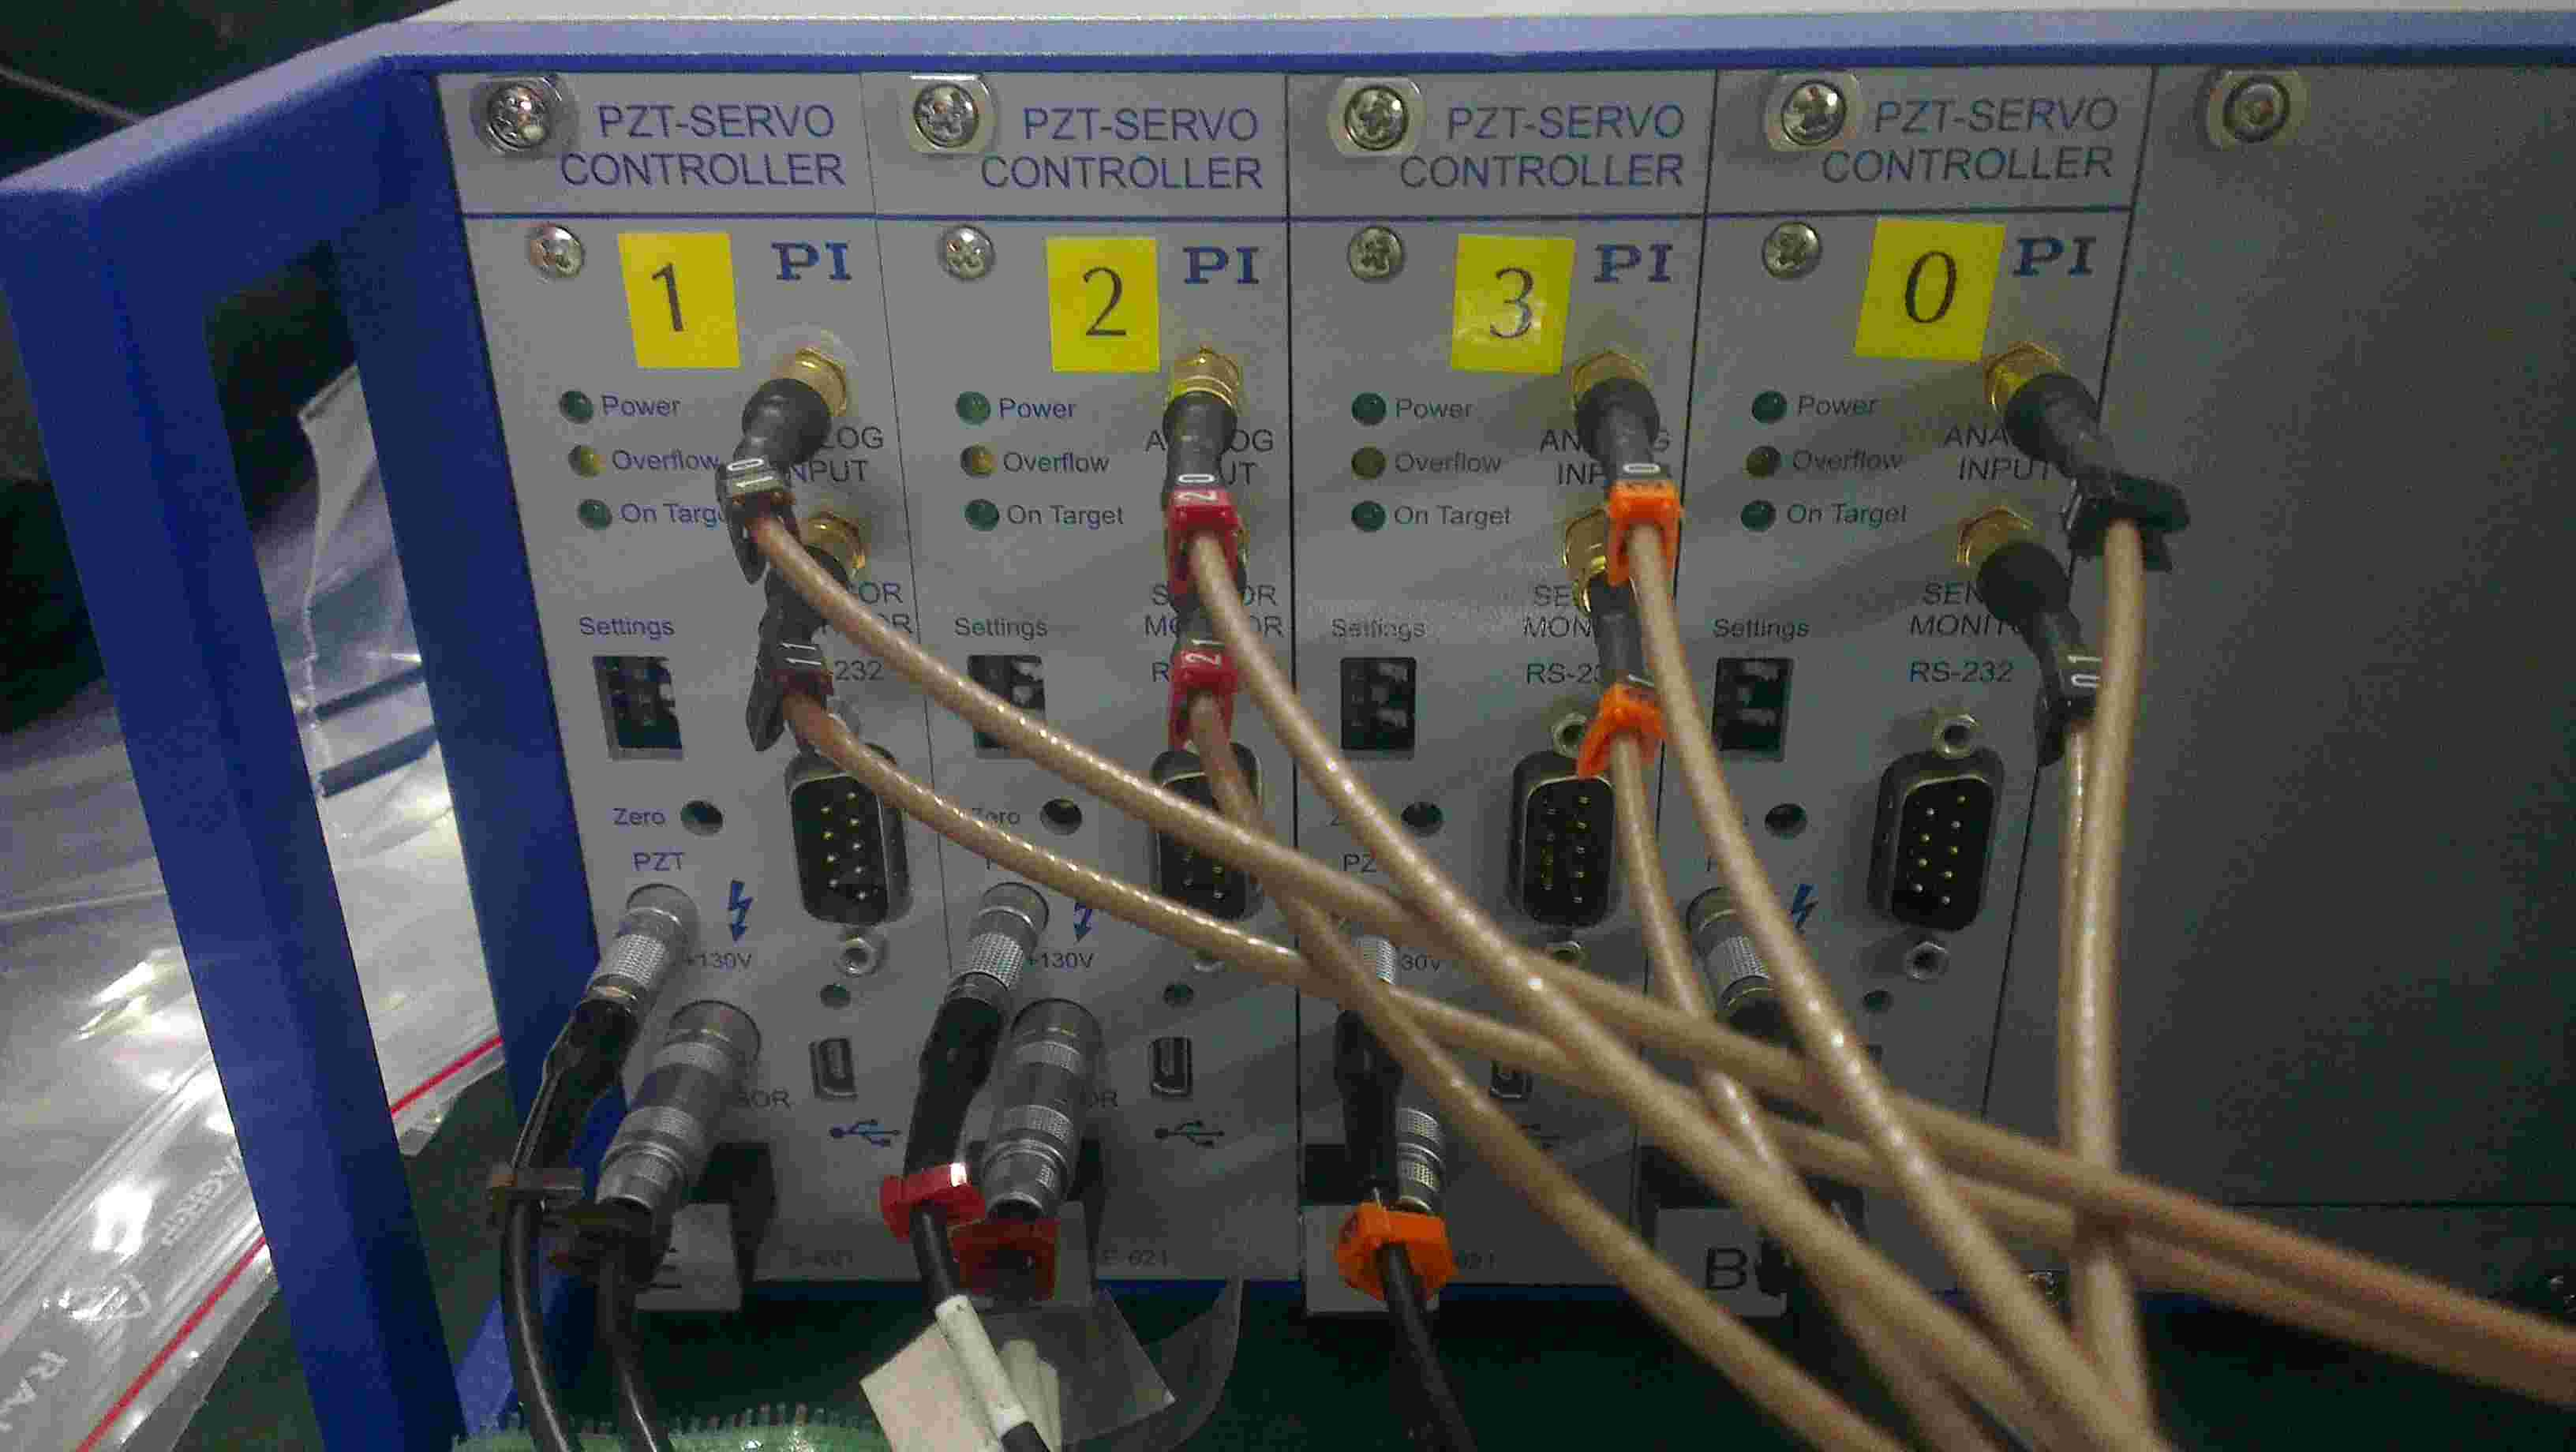
\includegraphics[height=1.6cm,width=3cm,angle=0]{ima04a.jpg}};
  \node (img5) at (2.0,0.0) {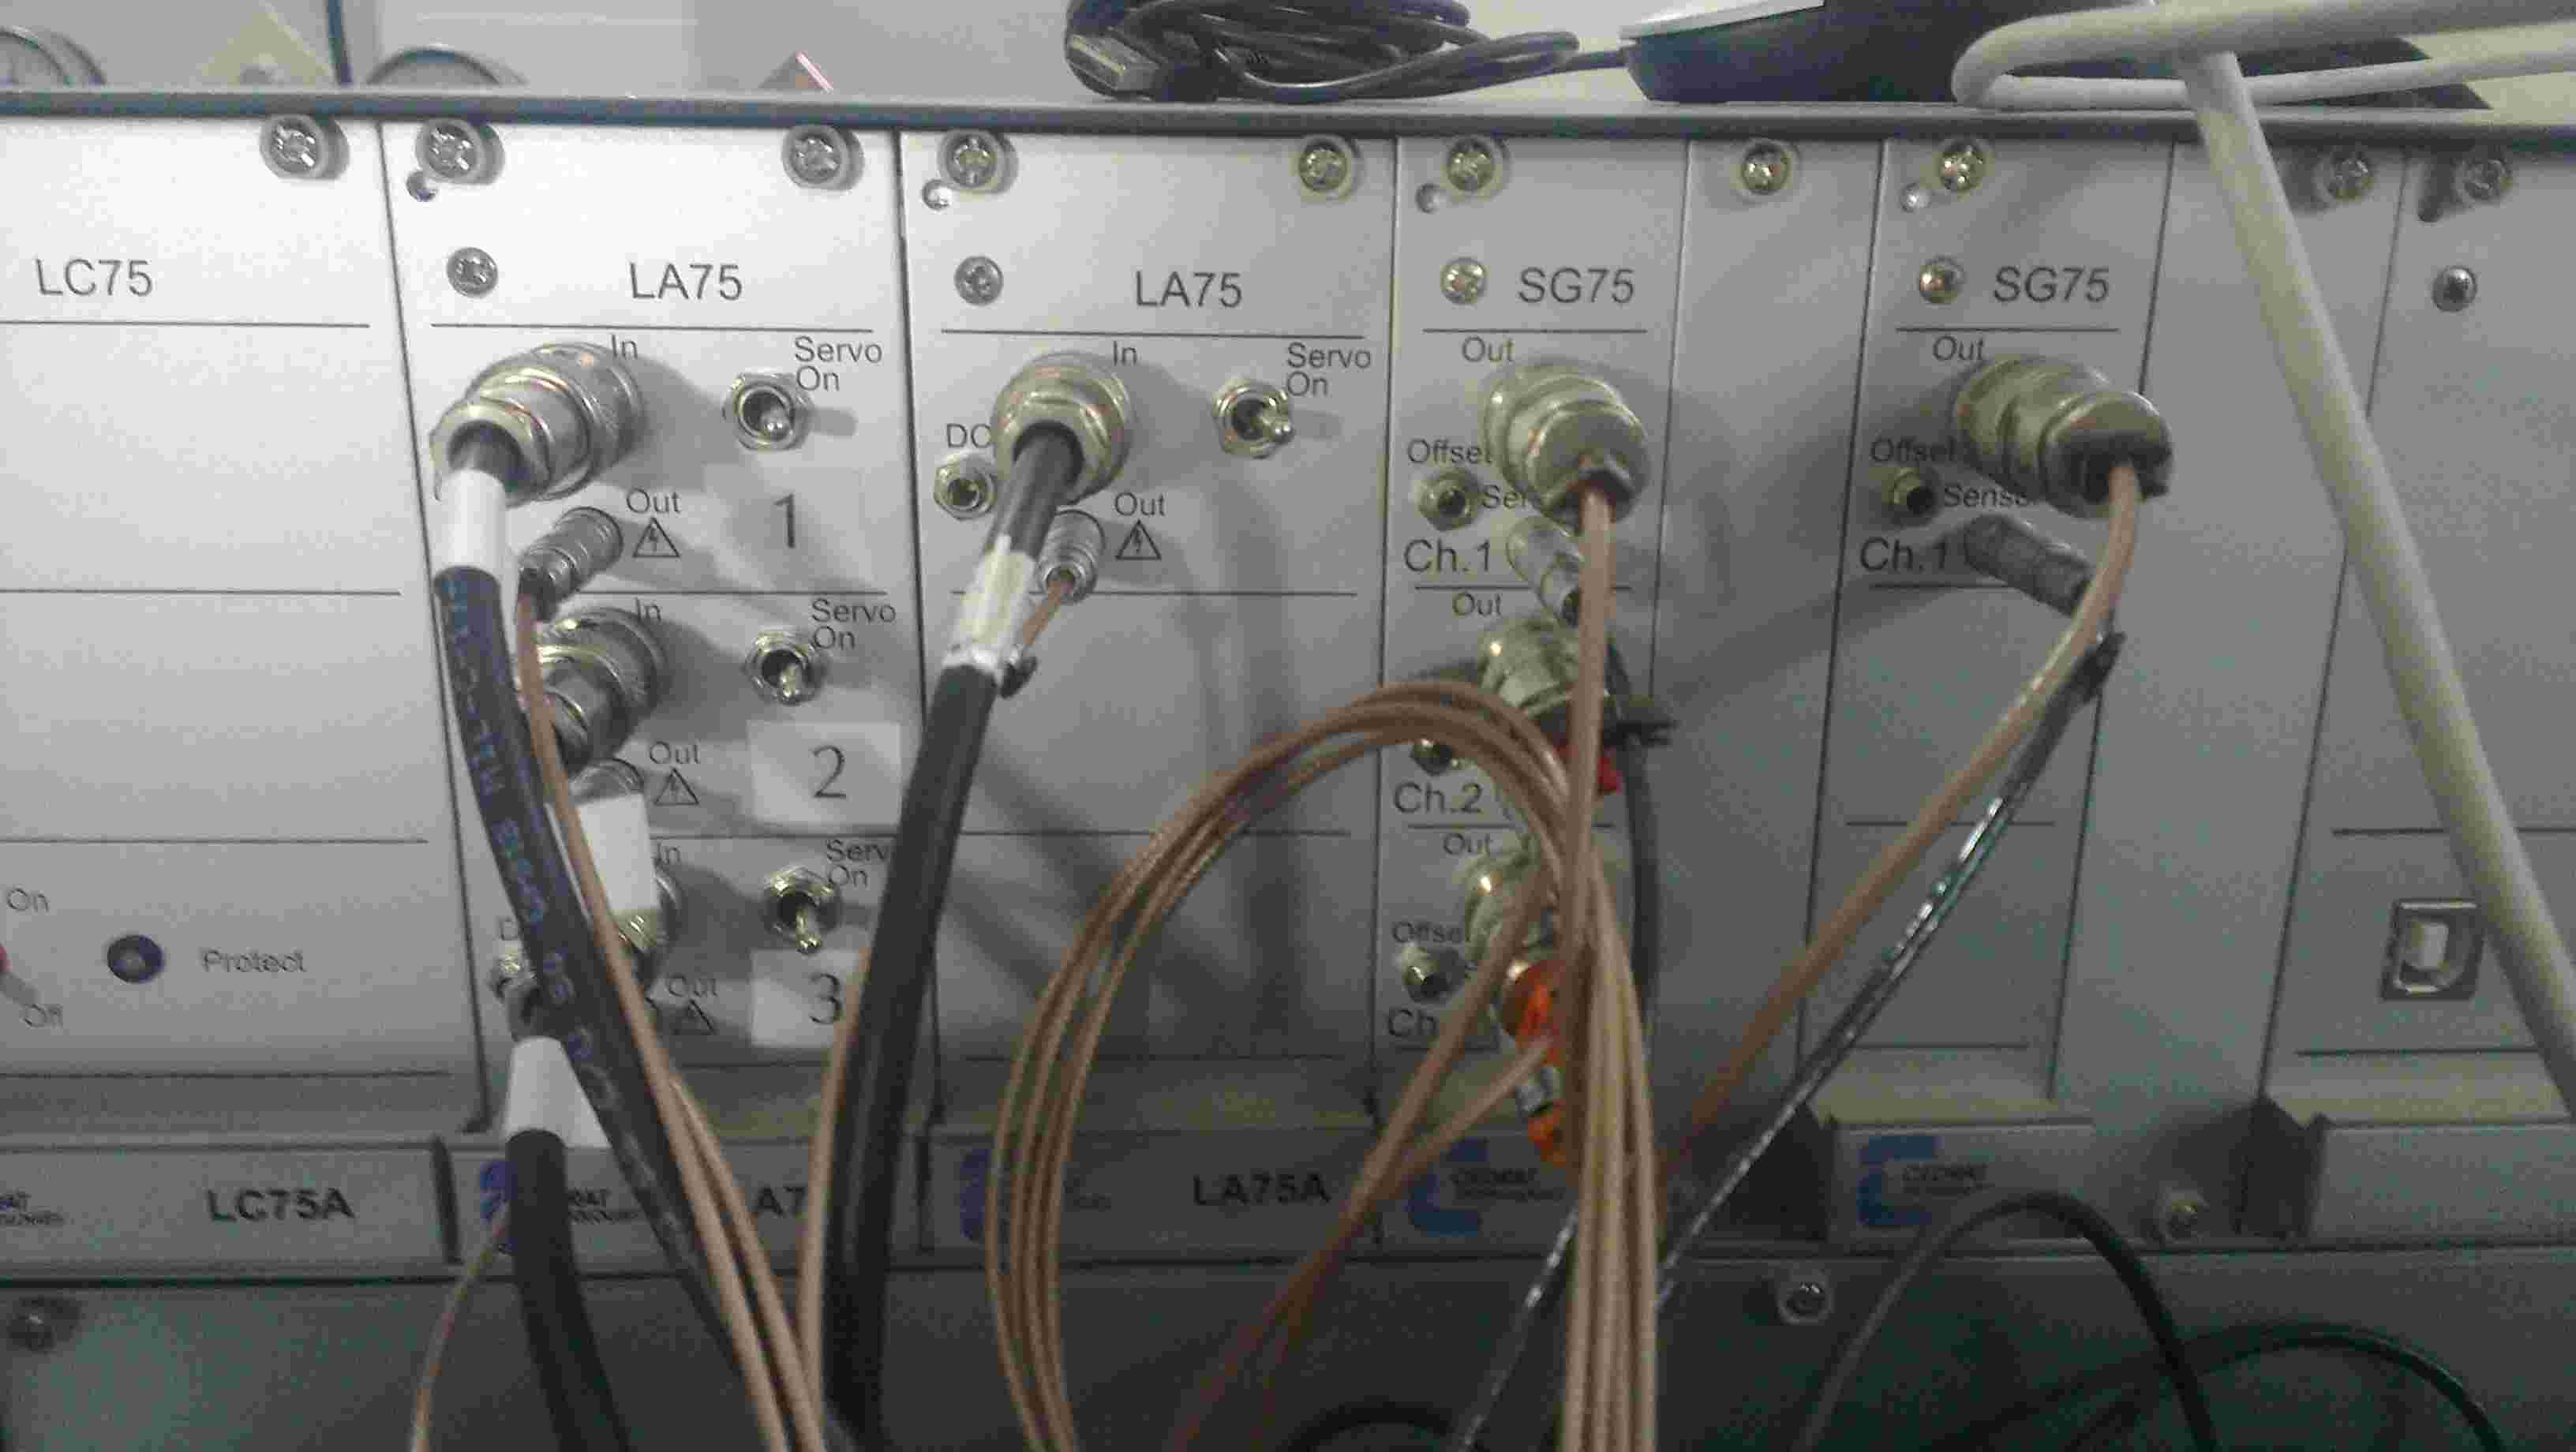
\includegraphics[height=1.6cm,width=3cm,angle=0]{ima05a.jpg}};
%   \pause
  \node (img6) at (4.4,3.0) {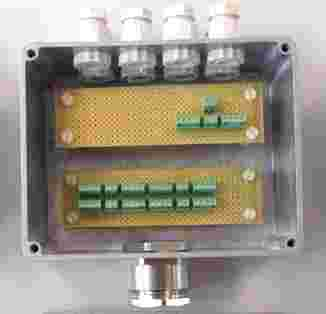
\includegraphics[height=1.6cm,width=3cm,angle=180]{ima08a.jpg}};
  \node (img7) at (1.8,1.4) {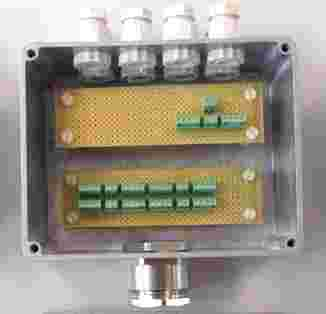
\includegraphics[height=1.6cm,width=3cm,angle=180]{ima08a.jpg}};
  \node (img8) at (1.8,3.0) {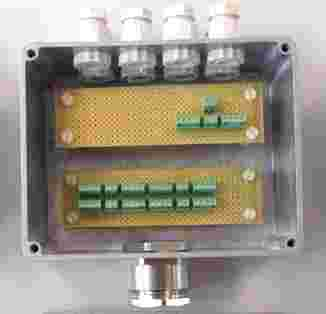
\includegraphics[height=1.6cm,width=3cm,angle=180]{ima08a.jpg}};
%   \pause
  \node (img9) at (-3.0,0.7)  {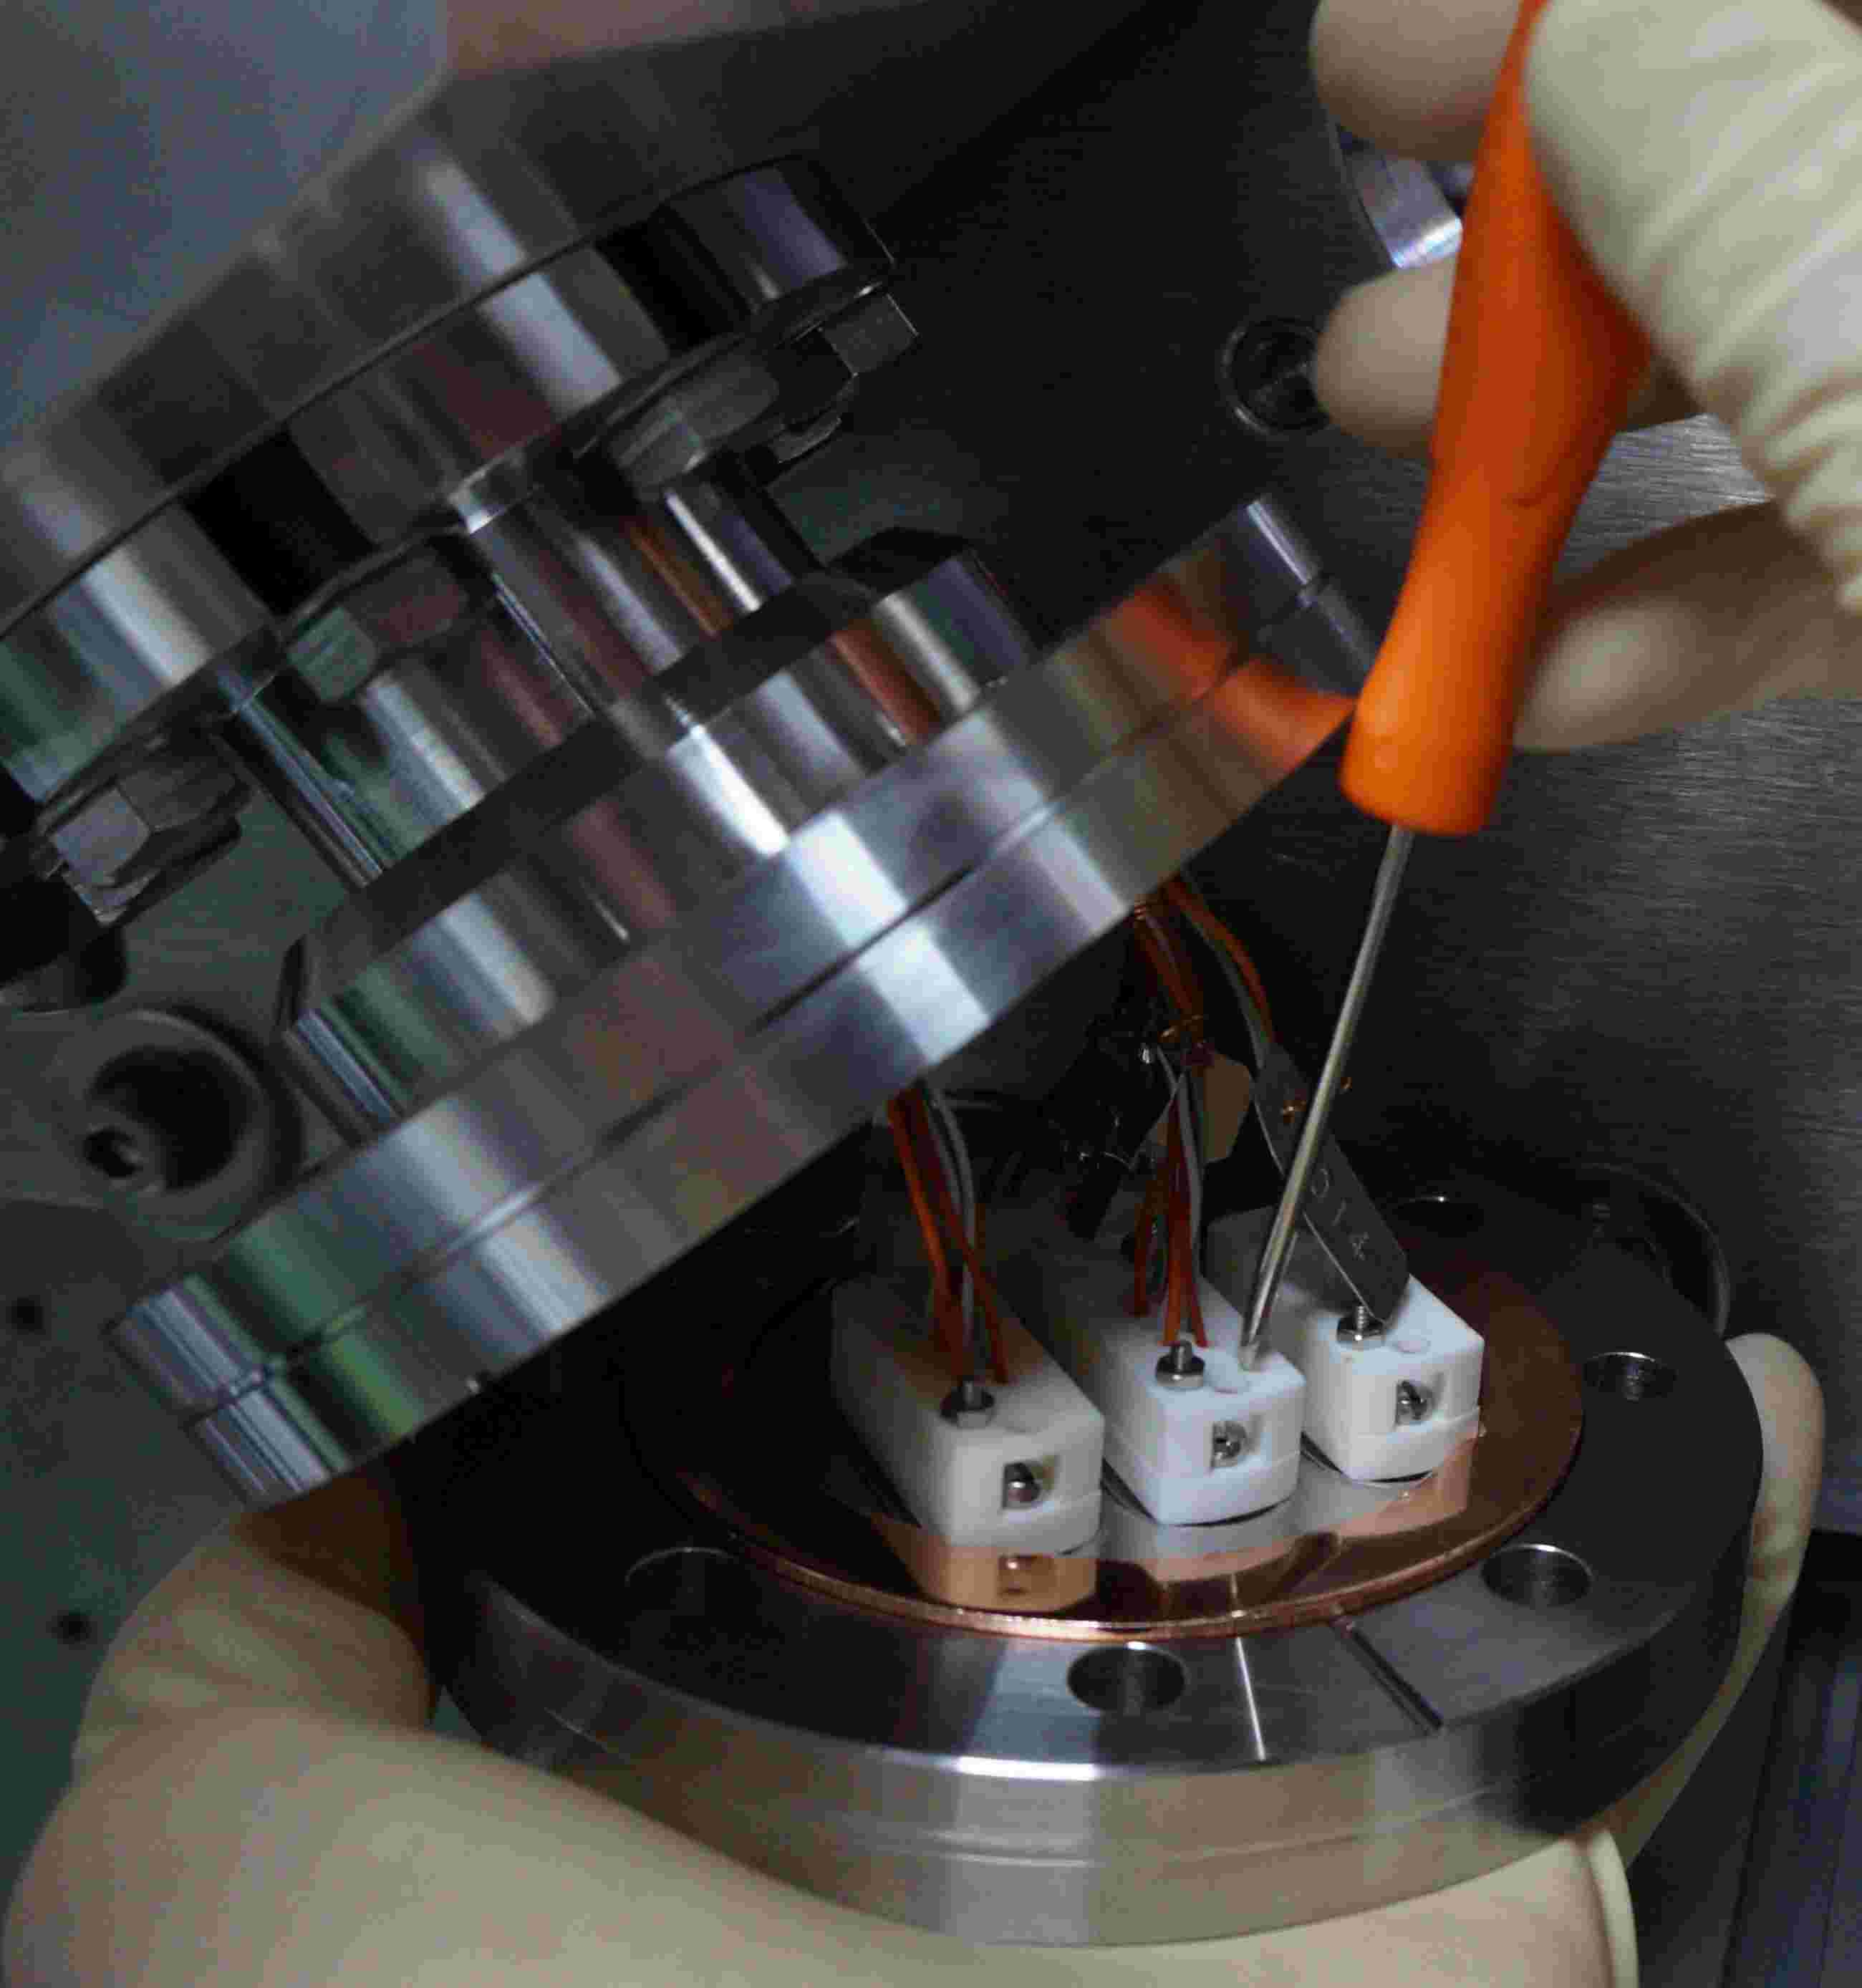
\includegraphics[height=1.6cm,width=1.4cm,angle=0]{ima10a.jpg}};
  \node (img10) at (-3.0,3.0) {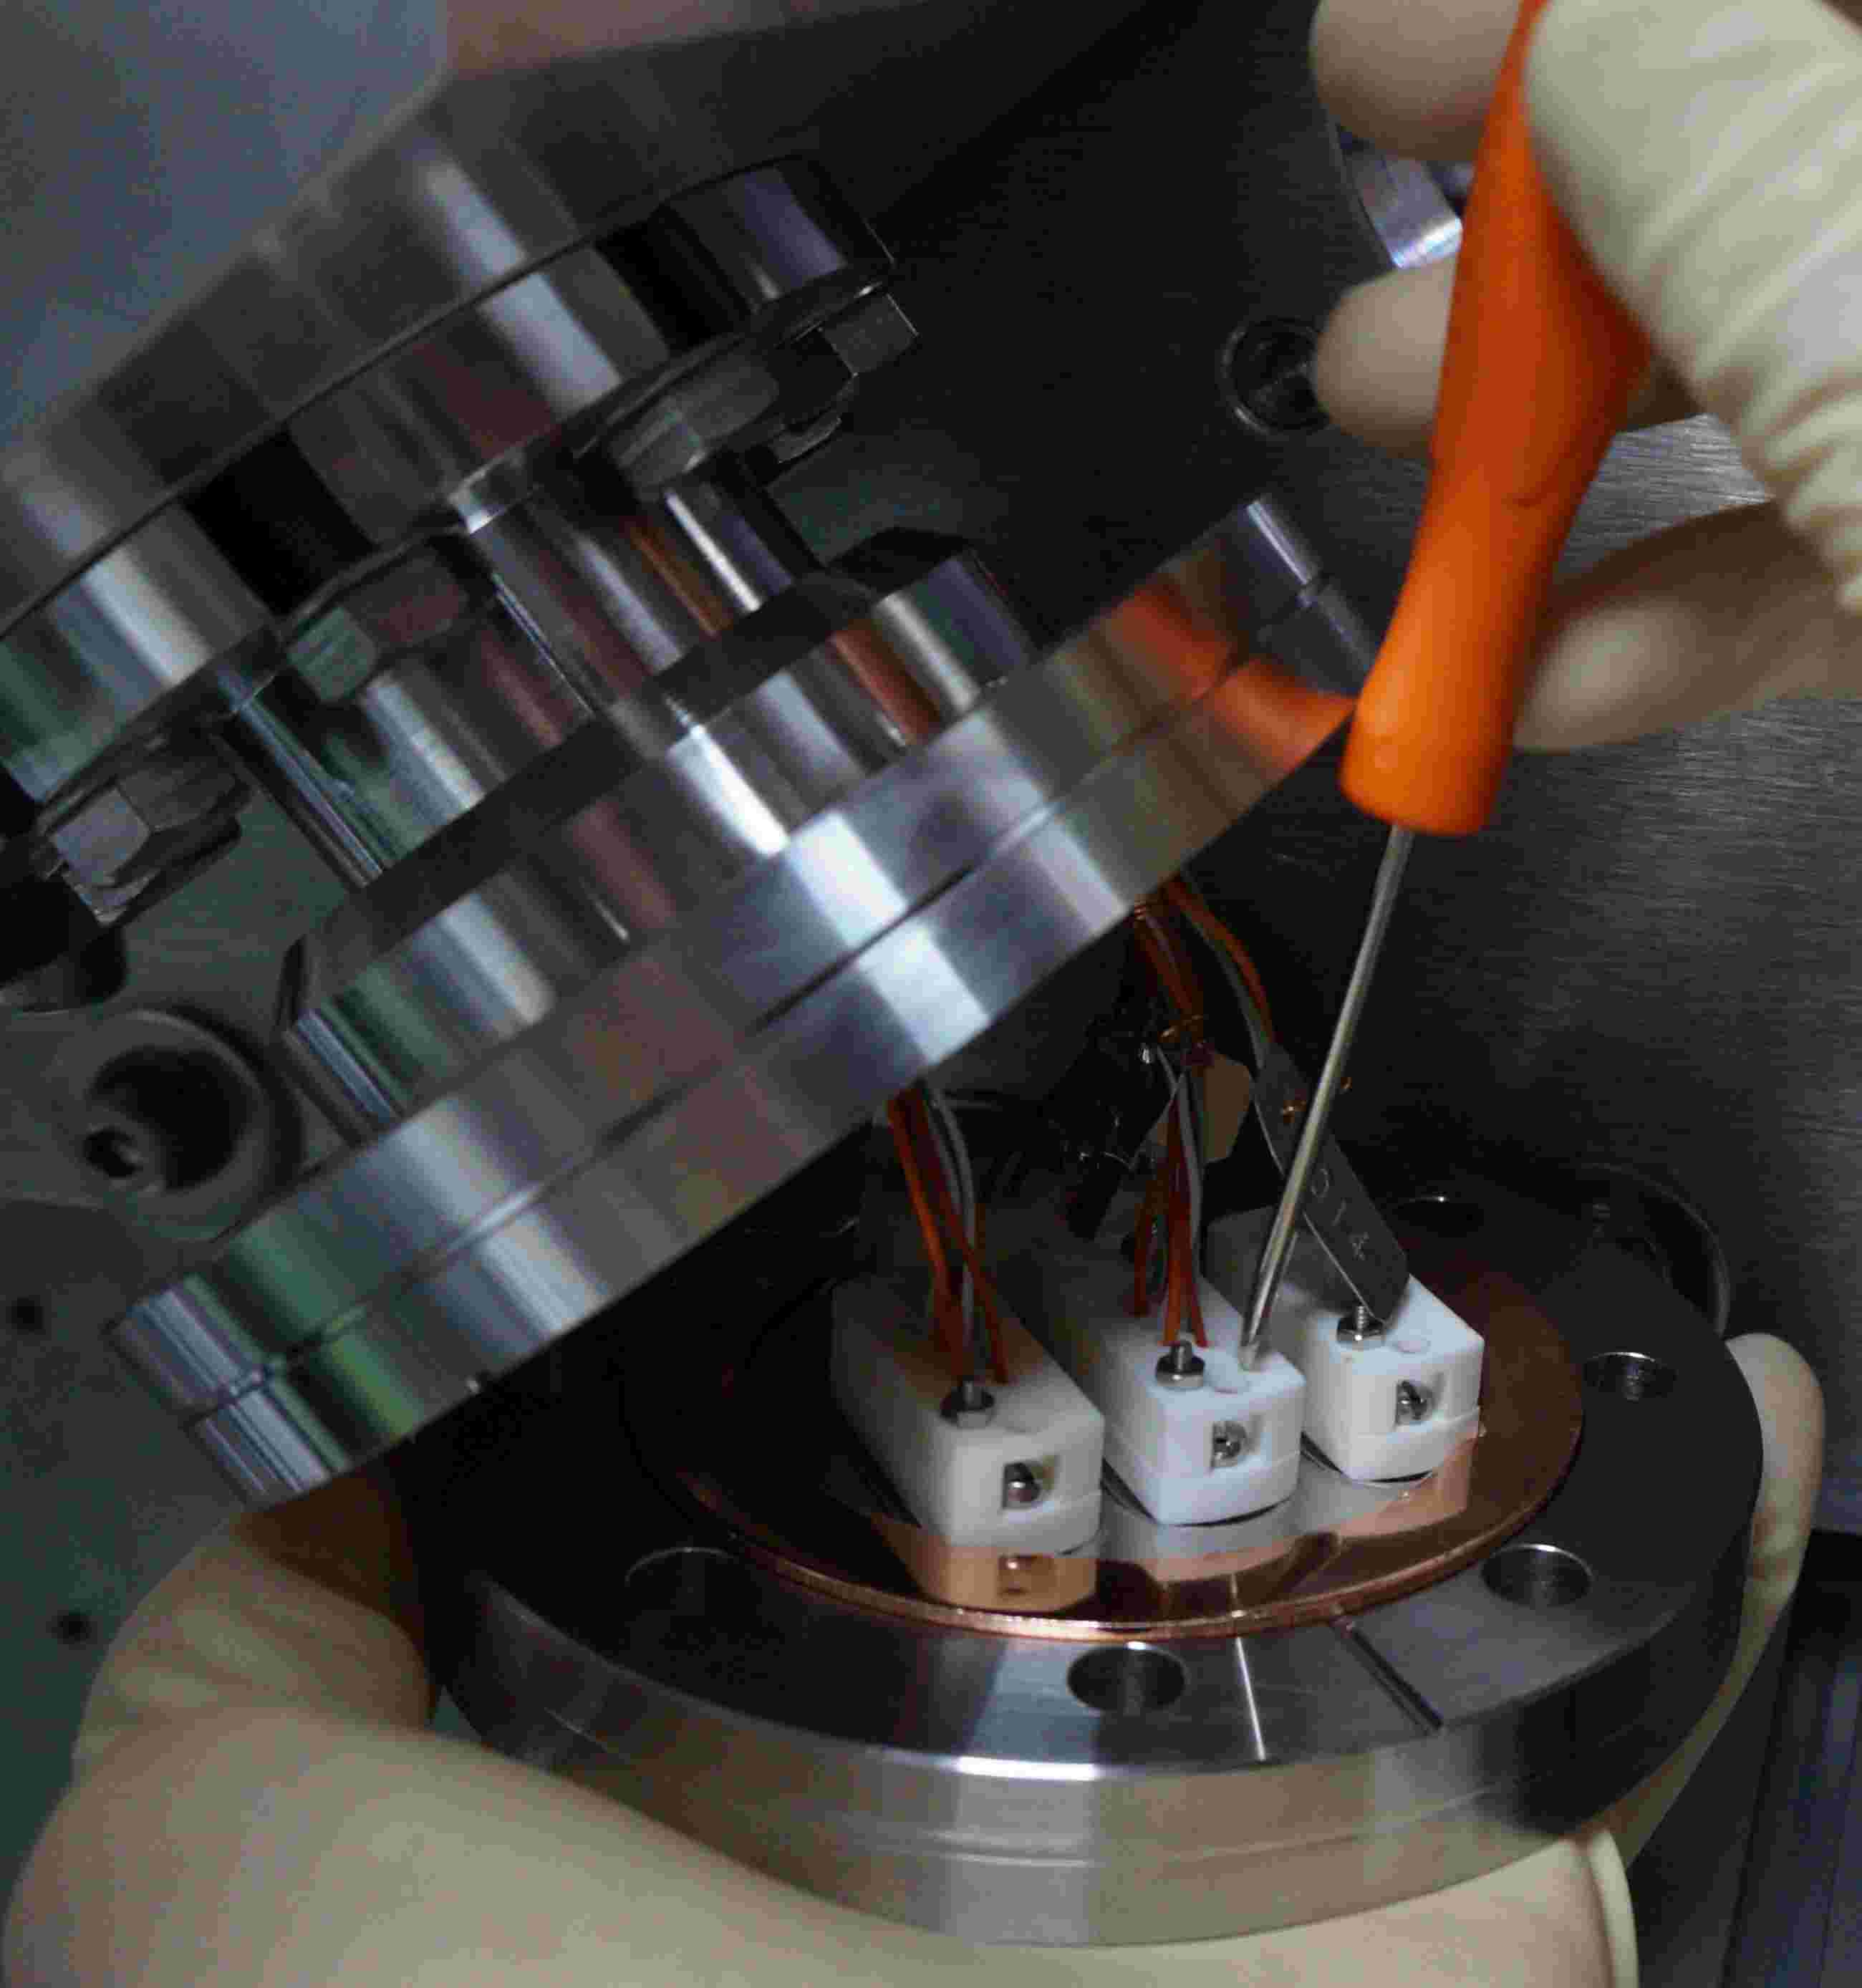
\includegraphics[height=1.6cm,width=1.4cm,angle=0]{ima10a.jpg}};
%   \pause
  \node (img11) at (-4.8,0.7)  {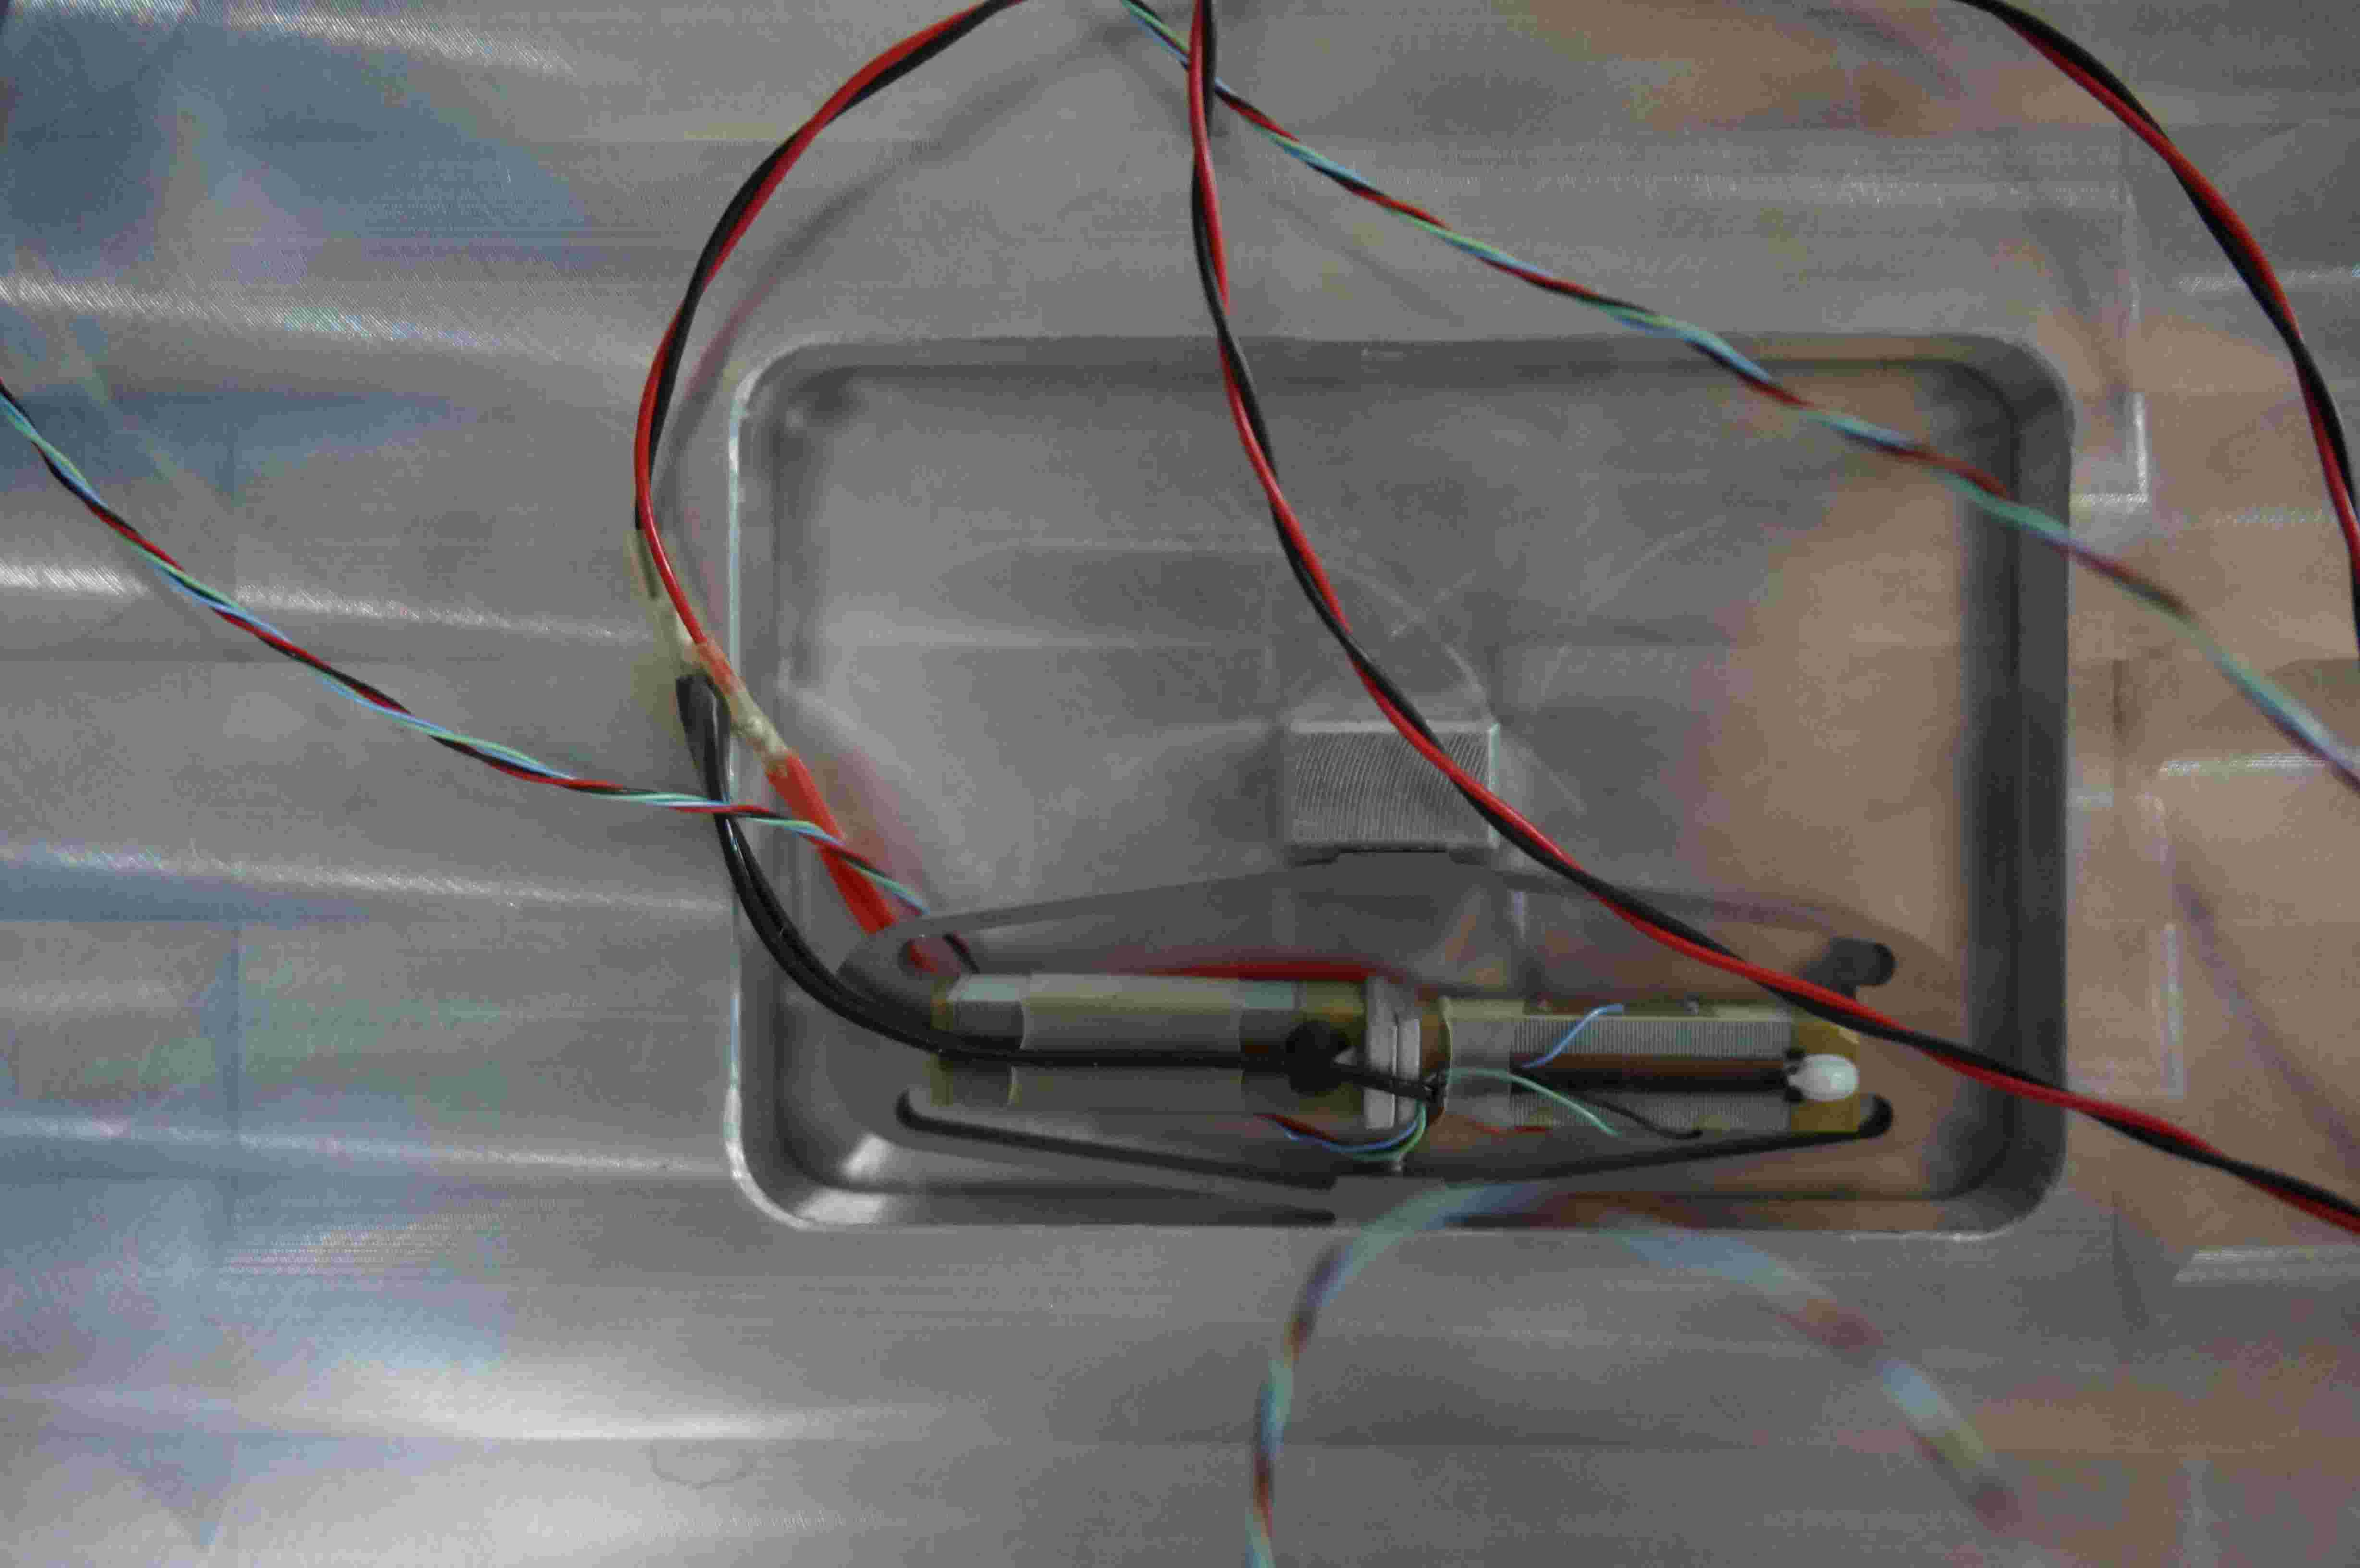
\includegraphics[height=1.6cm,width=1.4cm,angle=0]{ima11a.jpg}};
  \node (img12) at (-4.8,3.0) {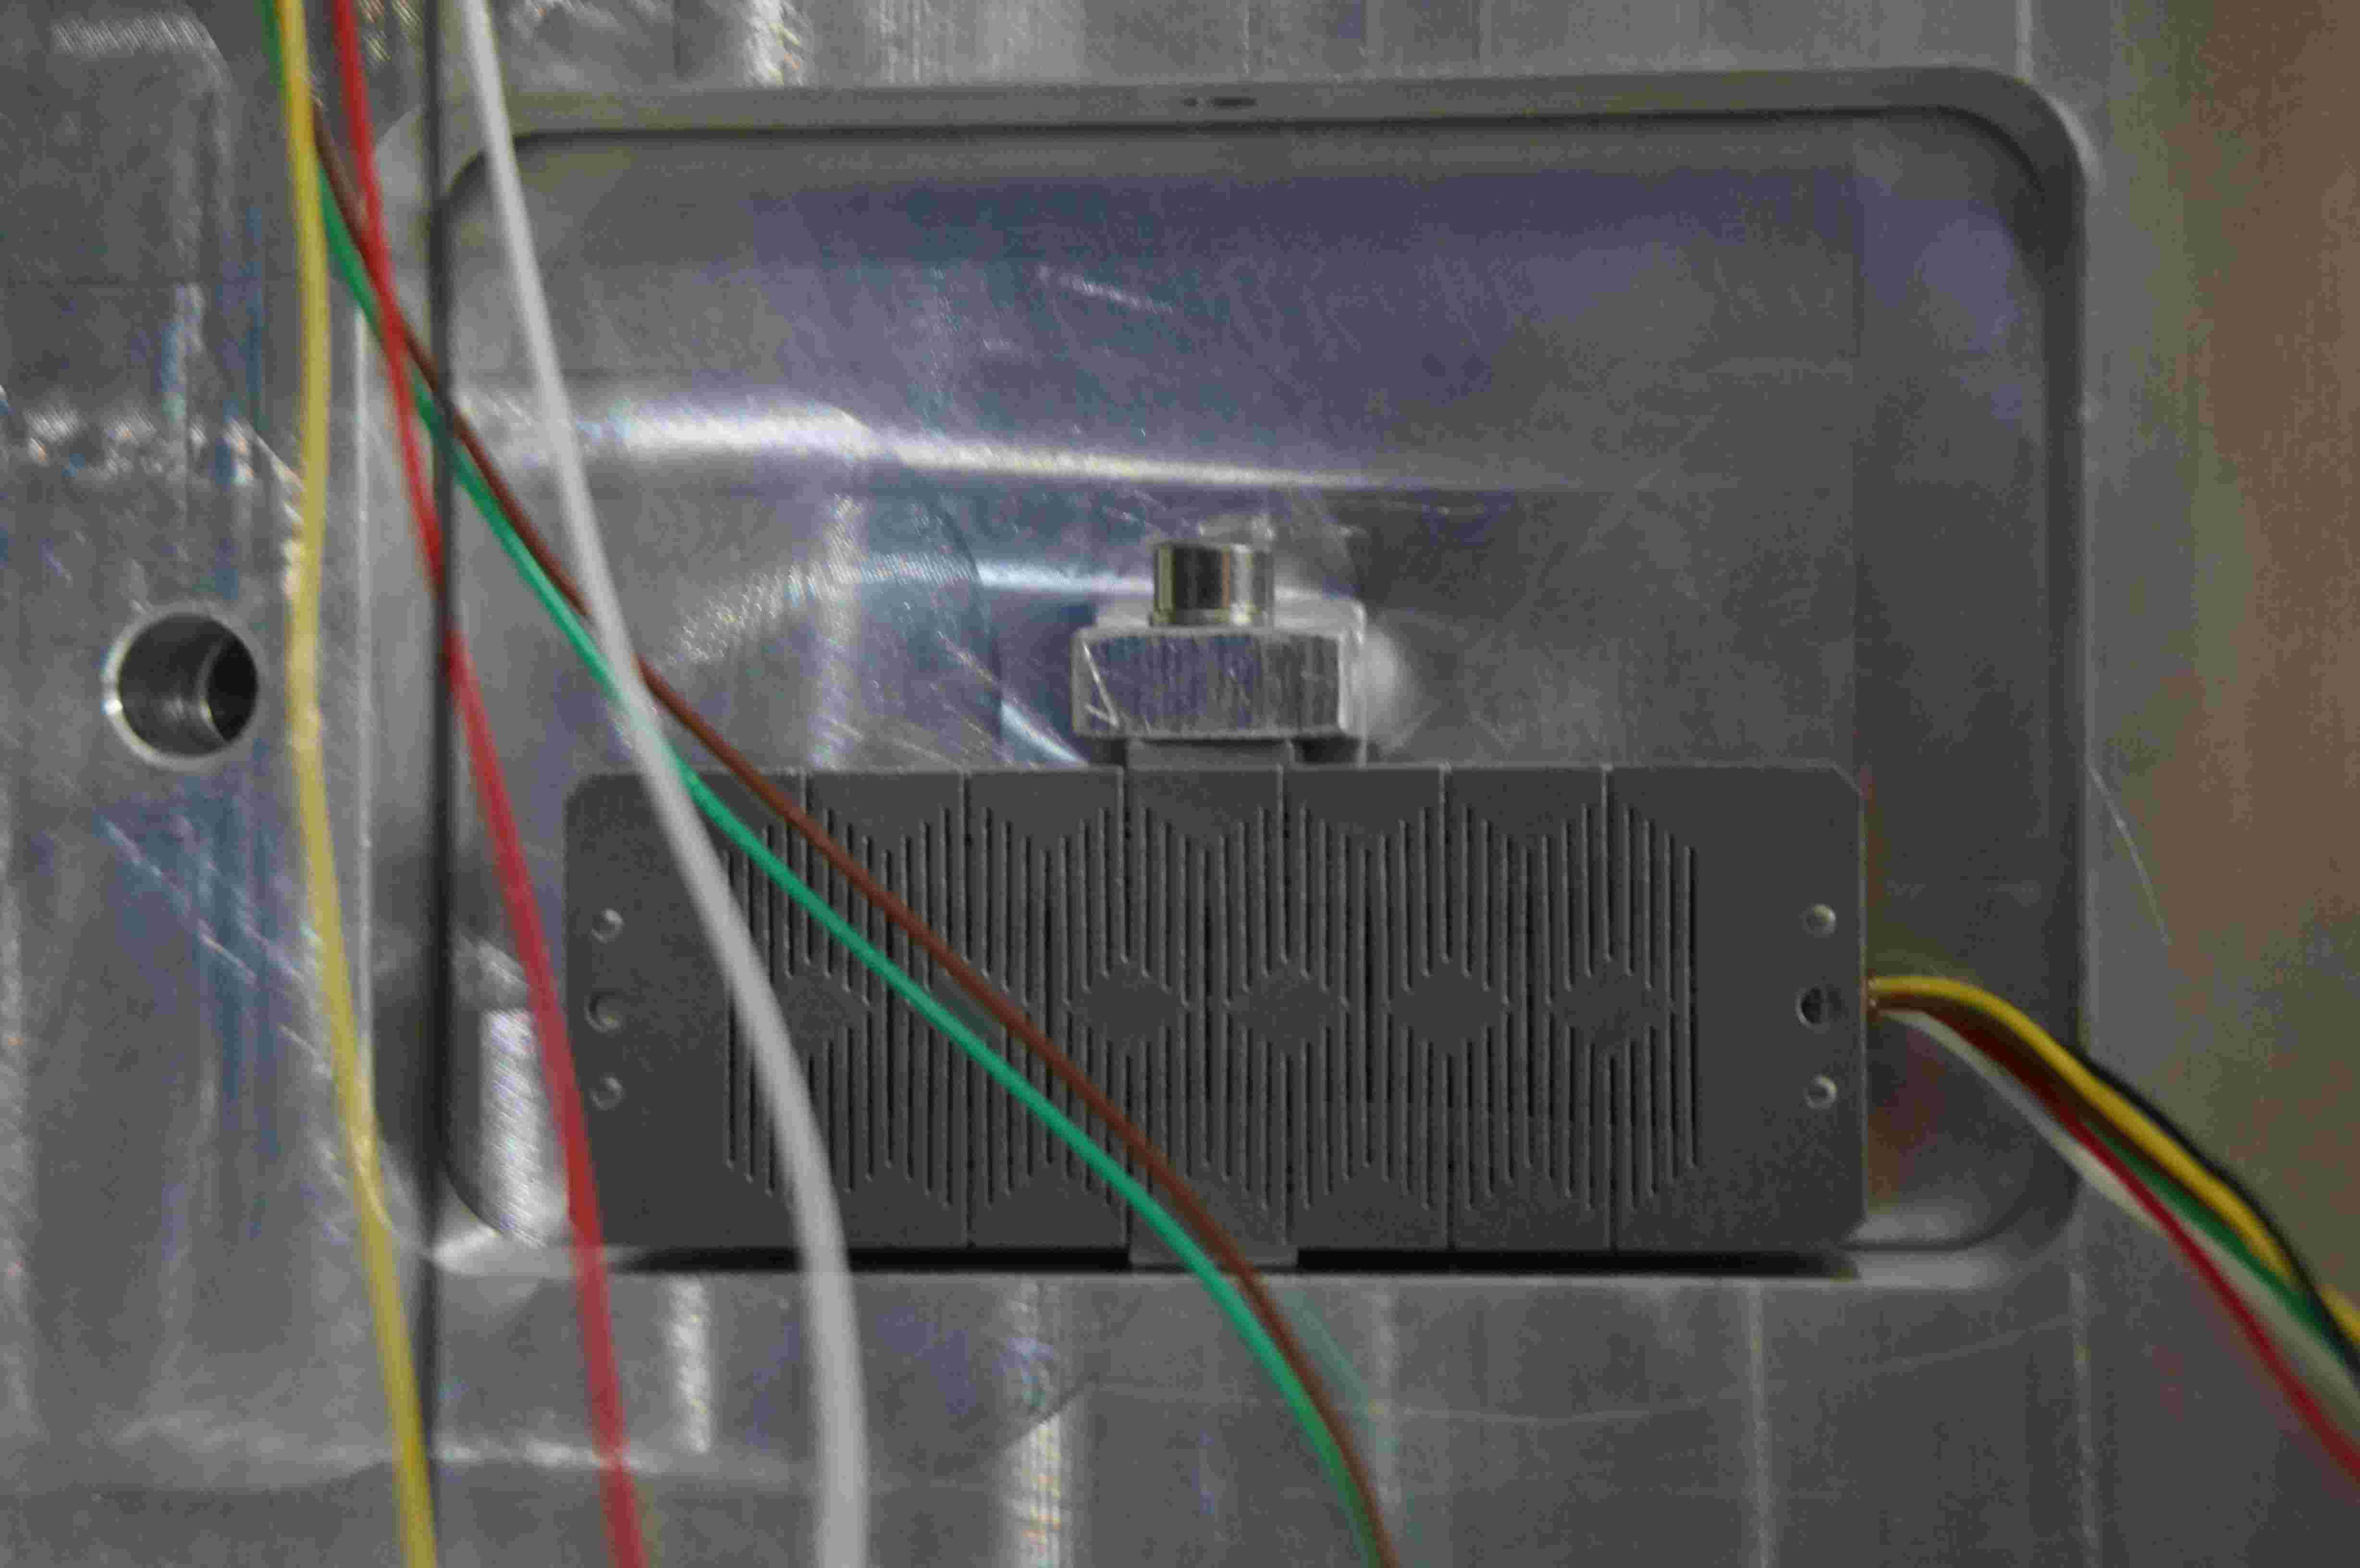
\includegraphics[height=1.6cm,width=1.4cm,angle=0]{ima12a.jpg}};
\end{tikzpicture}